\chapter{函数拟合与正则化}
\label{chap:opt-function-fitting}

在区间$[0,1]$上等距取$15$个点，读到一条曲线带误差的数值，现在要找一个函数“穿过”或“贴近”这些点。用$14$次多项式恰好穿过全部读数，方程有唯一解，可是图~\ref{fig:opt-fit-interpolation-vs-regularization}中的这条多项式在两端剧烈摆动，最高冲到$2.6$；同一组读数允许稍有偏差，同时惩罚曲率，得到的曲线平稳得多，最大值约$1.17$。两条曲线在观测点上都与数据相合或相近，在观测点之间却截然不同。读数没有说明点与点之间发生了什么，被选出的函数在那里的样子，完全取决于我们额外加进去的偏好和所用的求解过程。

\begin{figure}[!htbp]
  \centering
  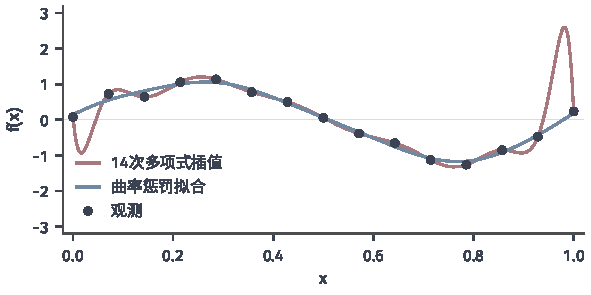
\includegraphics[width=100mm]{figures/03-optimization-evolution-and-signals/01-optimization/matplotlib/c8-interpolation-vs-regularization/figure.pdf}
  \caption{同一组读数上的插值与正则化拟合。教学示例数据为$x_i=i/14$（$i=0,\dots,14$），$y_i=\sin(2\pi x_i)+e_i$，$e_i$取自固定种子的$N(0,0.15^2)$。红线是穿过全部读数的$14$次多项式；蓝线在同一多项式空间中极小化$\sum_i(f(x_i)-y_i)^2+\lambda\int_0^1f''(x)^2\,\mathrm dx$，$\lambda=10^{-4}$。两者在观测点处取值相同或相近，在两端相差悬殊：前者的曲率积分约为$8.0\times10^{6}$，后者约为$1.2\times10^{3}$。}
  \label{fig:opt-fit-interpolation-vs-regularization}
\end{figure}

本章研究这样一类优化问题：未知量是一个函数，给定的是它的有限个读数，或者它在整个区域上带误差的取值、梯度。学习目标是回答四个问题。读数究竟约束了函数的哪些方向，哪些方向完全看不见；怎样用残差代价和正则化写出拟合目标，并把它变成可以计算的有限维问题；所得函数是否存在、是否唯一，又怎样求出来；输出对数据扰动、正则参数和有限计算有多敏感。我们只讨论确定性的拟合误差和数值误差，不把训练残差当作预测保证。

为与机器学习的惯用写法一致，本章改用拟合记号。数据是$n$对$(\bm x_i,y_i)$，读数向量$\bm y=(y_1,\dots,y_n)^\top$；候选函数记作$f$，观测映射记作$L$（本章中$L$专指观测，不表示梯度的Lipschitz常数）；把函数用固定基展开时，系数即参数$\bm w\in\mathbb R^d$，读数对系数的线性关系由设计矩阵$\bm X\in\mathbb R^{n\times d}$给出；非线性参数记作$\bm\theta$。于是前几章的决策变量$\bm x$在这里换成了$\bm w$或$\bm\theta$，而$\bm x_i$表示数据点的位置。

路线由“从有限到无限”的依赖决定。第一节先把观测、候选和误差的含义说清楚，区分数据本身的约束与额外的选解偏好。第二、三节在有限个参数中求解：线性参数下拟合目标是最小二乘或可由加权最小二乘逐轮处理的稳健目标，非线性参数下则先线性化残差，再用原目标检验步长。第四节转向无限维候选，表示定理说明有限个读数只需要在有限维子空间中搜索；第五节把观测扩大到整个区域上的函数值和梯度场，改用谱配方和闭子空间投影求解。前面得到的解都是某个精确问题的解，第六节比较数据扰动、正则参数和有限计算各自带来的偏差；第七节则说明当目标有许多最小点时，优化算法本身还会作出一次选择。

\section{观测与拟合目标}
\label{sec:opt-fit-observations}

章首的两条曲线说明，拟合问题至少由三样东西决定：允许选哪些函数，读到了函数的什么信息，以及读数与候选不完全相合时怎样计价。本节先把候选与观测写成数学对象，分清“数据能确定什么”与“我们额外偏好什么”；再比较几种残差代价与正则化；最后检查一个容易混淆的实例：把二次惩罚加进目标与在更新规则中直接收缩参数，是不是同一件事。

\subsection{有限观测与候选函数}
\label{sec:opt-fit-finite-observations}

\paragraph{候选集合与观测映射}
设我们在$x=0,\tfrac12,1$三处读到某个函数的值$0,1,0$。要从中“恢复”函数，先得说清从哪里找：可以是次数不超过$3$的多项式，也可以是$[0,1]$上所有连续函数，或某个函数空间。把允许的函数组成的集合称为候选集合，记作$C$。读数由一条规则从函数算出，这里是$f\mapsto(f(0),f(\tfrac12),f(1))$。一般地，称$L:C\to\mathbb R^n$，$Lf=(L_1f,\dots,L_nf)^\top$为\term{观测映射}（observation map），$\bm y\in\mathbb R^n$为数据，拟合就是在$C$中找$f$使$Lf$与$\bm y$相合或相近。

读数不必是点值。区间平均$L_if=(b-a)^{-1}\int_a^bf\,\mathrm dx$、加权积分$\int_0^1f\varphi_i\,\mathrm dx$都是关于$f$线性的读数，本章主要讨论这样的\emph{线性观测}：每个$L_i$对线性组合保持线性，$L_i(\alpha f+\beta g)=\alpha L_if+\beta L_ig$。

\paragraph{观测与候选空间必须相容}
同一条读取规则放在不同的候选空间里，可能根本没有意义。$L^2(0,1)$的元素是几乎处处相等的函数组成的等价类，改动一个点的值不改变元素本身，所以“在$x=\tfrac12$处取值”在$L^2(0,1)$上没有良定义。积分读数则不同：由Cauchy--Schwarz不等式，$\bigl|\int_a^bf\,\mathrm dx\bigr|\le\sqrt{b-a}\,\|f\|_{L^2}$，它在$L^2$上有定义且连续。若把候选放进再生核Hilbert空间$H_K$，点值读数满足$|f(x)|\le\sqrt{K(x,x)}\,\|f\|_{H_K}$，是有界线性泛函；这一性质以及核截面、Gram矩阵与核积分算子的谱展开，可参考\BookChapterRef{chap:rkhs}{卷二“再生核Hilbert空间”章}，本章第~\ref{sec:opt-fit-hilbert}节和第~\ref{sec:opt-fit-global}节会反复用到。所以写下拟合问题之前，先要核对每个$L_i$在$C$上是否有定义，必要时是否连续。

\paragraph{有解、唯一与可识别}
给定观测映射以后，有三个不同的问题。第一，方程$Lf=\bm y$在$C$中是否有解，即$\bm y$是否属于像集$L(C)$。第二，对这一组具体数据，解是否唯一。第三，不论数据取什么值，$L$在$C$上是否单射，即读数是否总能区分两个不同的候选。前两个问题依赖于$\bm y$，第三个只依赖于$C$与$L$。

\begin{lemma}[读数区分全部候选的条件]
\label{lem:opt-fit-identifiability}
设$C$是线性空间$V$的子集，$L:V\to\mathbb R^n$线性。记$C-C=\{f-g:f,g\in C\}$。则$L$在$C$上单射，当且仅当$(C-C)\cap\ker L=\{0\}$。
\end{lemma}

\begin{proof}
对$f,g\in C$，由线性，$Lf=Lg$当且仅当$f-g\in\ker L$。若$(C-C)\cap\ker L=\{0\}$，则$Lf=Lg$推出$f-g=0$。反之，若有非零的$f-g\in(C-C)\cap\ker L$，则$f\ne g$而$Lf=Lg$，单射不成立。
\end{proof}

当$C$本身是线性子空间时，$C-C=C$，条件化为$C\cap\ker L=\{0\}$。取$C$为次数不超过$3$的多项式，三个点值读数不能区分全部候选：$p(x)=x(x-\tfrac12)(x-1)$非零，却在三个观测点处都等于零。于是$f_0(x)=4x(1-x)$与$f_0+c\,p$对每个实数$c$都给出同样的读数$(0,1,0)$。图~\ref{fig:opt-fit-invisible-direction}画出了$c=0,\pm8,\pm16$的五条曲线：它们在三个黑点处重合，在点与点之间沿$p$的方向任意偏移。$p$所在的方向对这组读数完全不可见。

\begin{figure}[!htbp]
  \centering
  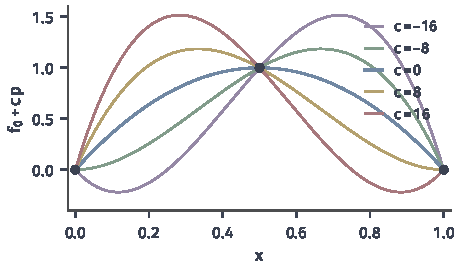
\includegraphics[width=78mm]{figures/03-optimization-evolution-and-signals/01-optimization/matplotlib/c8-invisible-direction/figure.pdf}
  \caption{观测不可见的方向。在次数不超过$3$的多项式中，$f_0(x)=4x(1-x)$与$f_0+c\,p$（$p(x)=x(x-\tfrac12)(x-1)$，$c=0,\pm8,\pm16$）在$x=0,\tfrac12,1$处的读数都是$0,1,0$（黑点）。$p$属于观测映射的零空间，读数无法区分这些候选。}
  \label{fig:opt-fit-invisible-direction}
\end{figure}

\paragraph{惩罚只提供选解偏好}
在这条直线$\{f_0+c\,p:c\in\mathbb R\}$上，若偏好“弯曲最少”的函数，可以比较曲率积分$\int_0^1(f'')^2\,\mathrm dx$。由$f_0''=-8$、$p''=6x-3$，
\[
  \begin{aligned}
  \int_0^1\bigl(-8+c(6x-3)\bigr)^2\,\mathrm dx
  &=64-16c\int_0^1(6x-3)\,\mathrm dx+c^2\int_0^1(6x-3)^2\,\mathrm dx\\
  &=64+3c^2,
  \end{aligned}
\]
所以惩罚选出$c=0$，即$f_0$。这个选择来自惩罚，而不是来自数据：读数对所有$c$都一样，数据既不支持也不反对$c=0$。换一种惩罚，例如偏好$f(\tfrac14)$接近某个值，就可能选出另一个$c$。正则化可以在观测无法区分的候选之间作出确定的选择，却不能增加读数本身的识别能力。

\subsection{残差、正则化与插值}
\label{sec:opt-fit-residual-regularization}

\paragraph{残差的计价方式}
读数带有误差时，强求$Lf=\bm y$可能既不可能也不合理，于是改为允许残差$\bm r=Lf-\bm y$，并给残差计价。常用的三种代价是平方$r^2/2$、绝对值$|r|$，以及在两者之间过渡的\term{Huber损失}（Huber loss）\scite{huber1964}
\[
  h_\delta(r)=
  \begin{cases}
    r^2/2,&|r|\le\delta,\\
    \delta|r|-\delta^2/2,&|r|>\delta,
  \end{cases}
\]
其中$\delta>0$是转折尺度。图~\ref{fig:opt-fit-residual-losses}(a)比较了它们的形状：平方代价对大残差按平方增长，绝对值只按线性增长，Huber损失在$|r|\le\delta$内与平方相同、在外与绝对值平行。图中还画了按对数增长的Cauchy代价$\tfrac12\log(1+r^2)$，第~\ref{sec:opt-fit-irls}小节会用到它。

\begin{figure}[!htbp]
  \centering
  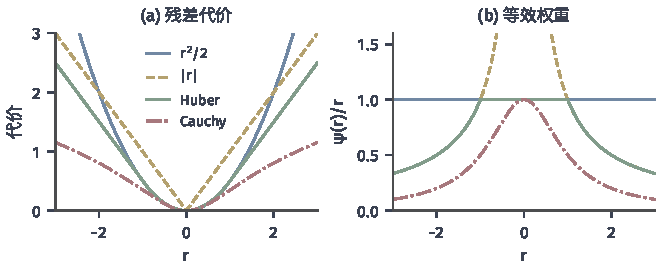
\includegraphics[width=112mm]{figures/03-optimization-evolution-and-signals/01-optimization/matplotlib/c8-residual-losses/figure.pdf}
  \caption{残差代价及其等效权重。(a)~平方$r^2/2$、绝对值$|r|$、Huber损失（$\delta=1$）与Cauchy代价$\tfrac12\log(1+r^2)$。(b)~把每种代价写成$\tfrac12\rho(r^2)$后的权重$\rho'(r^2)=\psi(r)/r$，其中$\psi$是代价对$r$的导数：平方代价对所有残差权重为$1$，绝对值的权重$1/|r|$在零残差处无界，Huber权重为$\min\{1,1/|r|\}$，Cauchy权重$1/(1+r^2)$随残差增大趋于零。}
  \label{fig:opt-fit-residual-losses}
\end{figure}

计价方式直接改变答案。用一个常数$w$拟合三个读数$0,0,10$：平方代价$\sum_i(w-y_i)^2/2$在均值$w=10/3$处最小；绝对值代价$\sum_i|w-y_i|$在中位数$w=0$处最小；对$\delta=1$的Huber损失，若$0\le w\le1$，前两项各为$w^2/2$，第三项为$(10-w)-\tfrac12$，和为$w^2-w+9.5$，在$w=\tfrac12$处导数为零，而目标是凸的，所以$w=\tfrac12$是全局最小点。远离其他读数的$10$把均值拉到$10/3$，对Huber解只施加了大小为$\delta$的有界推力。

每个读数还可以带一个给定的正权重$\omega_i$，表示我们对该读数的信任程度，此时数据代价写成$\sum_i\omega_i\ell(r_i)$。本章把$\omega_i$当作事先确定的量；怎样由噪声的统计模型推出损失与权重，属于统计推断的问题，可参考\BookChapterRef{chap:statistical-inference}{卷四“统计推断”章}。

\paragraph{插值与拟合是不同的任务}
要求$Lf=\bm y$精确成立的任务称为\term{插值}（interpolation），它把读数当作硬约束；允许残差并为之计价的任务称为拟合。前者在读数不相容时无解，后者总可以写出目标值。两者的解一般也不同，第~\ref{sec:opt-fit-min-norm-interpolation}小节会给出插值有解的判据，并说明不能用最小二乘解冒充插值。

\paragraph{一般的拟合目标}
把上面的成分合在一起，拟合问题写作
\begin{equation}
  \min_{f\in C}\ \Phi(Lf-\bm y)+\lambda R(f),
  \label{eq:opt-fit-general-objective}
\end{equation}
其中$\Phi:\mathbb R^n\to\mathbb R$是数据代价，例如$\Phi(\bm r)=\sum_i\omega_i\ell(r_i)$；$R:C\to[0,+\infty]$是\term{正则化}（regularization）项，表达读数之外的偏好；$\lambda\ge0$称为\term{正则化参数}（regularization parameter），调节两者的相对分量；候选集合$C$本身还可以包含硬约束，例如$f\ge0$或固定的边界值。插值则写成$\min_{f\in C}R(f)$，s.t.\ $Lf=\bm y$。数据代价、正则化和硬约束分别承担不同的职责，不能互相替代。

\paragraph{不同的正则化控制不同的东西}
以一次函数$f(x)=w_1+w_2x$为例，三种看似相近的“范数”惩罚的是不同的量。系数的欧氏范数$w_1^2+w_2^2$依赖于基的选取，换成基$\{1,x-\tfrac12\}$就会改变；$L^2$范数$\int_0^1f^2\,\mathrm dx=w_1^2+w_1w_2+w_2^2/3$度量函数本身的大小；导数半范数$\int_0^1(f')^2\,\mathrm dx=w_2^2$只惩罚斜率，对所有常数函数都等于零。最后一种是\term{半范数}（seminorm）：它满足齐次性与三角不等式，却在非零的常数上取零，因此单独使用时不会限制函数的整体高度。第~\ref{sec:opt-fit-linear-basis}小节将看到，在同一组数据上这三种惩罚会选出不同的函数。

\paragraph{有限正则参数不等于精确约束}
有人把约束$Lf=\bm y$换成罚项$\rho\|Lf-\bm y\|_2^2$，期望在$\rho$足够大时得到同样的解。一维例子说明这一般不成立：在约束$w=1$下极小化$w^2$，答案是$w=1$；而$w^2+\rho(w-1)^2$的极小点是$w=\rho/(1+\rho)$，对任何有限的$\rho>0$都严格小于$1$。罚项只能在极限$\rho\to\infty$下逼近约束，有限的正则参数对应的是另一个问题。

\subsection{显式正则化与参数衰减}
\label{sec:opt-fit-weight-decay}

上一小节把偏好写进目标~\eqref{eq:opt-fit-general-objective}。训练神经网络时还有另一种常见做法：目标只含数据项，而在每次更新时把参数乘以略小于$1$的因子。两种做法都叫“正则化”，它们是否等价？本小节在同一个数据目标$F(\bm w)$上逐项比较。

\paragraph{两种更新规则}
Adam维护一阶与二阶历史统计$\bm m,\bm v$，以衰减系数$\beta_1,\beta_2\in[0,1)$更新，并做零初始化的偏差校正，其构造见第~\ref{chap:opt-stochastic-block}章；这里只需要它的一轮更新形式。记第$t$轮（$t=1,2,\dots$）读入的方向为$\bm g^{(t)}$，所有平方、开方与除法逐坐标进行：
\[
  \begin{gathered}
  \bm m^{(t)}=\beta_1\bm m^{(t-1)}+(1-\beta_1)\bm g^{(t)},\qquad
  \bm v^{(t)}=\beta_2\bm v^{(t-1)}+(1-\beta_2)(\bm g^{(t)})^2,\\
  \widehat{\bm m}=\frac{\bm m^{(t)}}{1-\beta_1^t},\qquad
  \widehat{\bm v}=\frac{\bm v^{(t)}}{1-\beta_2^t}.
  \end{gathered}
\]
第一种做法把$\tfrac\lambda2\|\bm w\|_2^2$加进目标，于是$\bm g^{(t)}=\nabla F(\bm w^{(t-1)})+\lambda\bm w^{(t-1)}$，更新为$\bm w^{(t)}=\bm w^{(t-1)}-\eta\,\widehat{\bm m}/(\sqrt{\widehat{\bm v}}+\varepsilon)$。第二种做法是AdamW\scite{loshchilov2019adamw}，称为\term{解耦权重衰减}（decoupled weight decay）：统计只读取数据梯度$\bm g^{(t)}=\nabla F(\bm w^{(t-1)})$，衰减另外施加，
\begin{equation}
  \bm w^{(t)}=(1-\eta\lambda)\bm w^{(t-1)}-\eta\,\frac{\widehat{\bm m}}{\sqrt{\widehat{\bm v}}+\varepsilon}.
  \label{eq:opt-fit-adamw}
\end{equation}
这里约定两项都由更新前的参数与本轮统计算出。若先完成梯度步、再把整个结果乘以$1-\eta\lambda$，梯度项也会被缩放，得到的是另一条更新规则；两者共用“权重衰减”这个名称，却不能混用。

\paragraph{一个可复算的首步}
取标量参数$w^{(0)}=1$，两个历史矩为零，数据梯度恒为零，$\eta=0.1$，$\lambda=2$，$\varepsilon=1$。AdamW的统计只看到零梯度，$\widehat m=0$，由式~\eqref{eq:opt-fit-adamw}，$w^{(1)}=(1-0.2)\cdot1=0.8$。把二次正则加入目标后，$g^{(1)}=\lambda w^{(0)}=2$，偏差校正给出$\widehat m=2$、$\widehat v=4$，于是$w^{(1)}=1-0.1\cdot2/(2+1)=14/15$。同一个$\lambda$，两种做法在第一步就给出不同的结果。

图~\ref{fig:opt-fit-decay-vs-l2}(a)把这一比较延续到$30$步（$\beta_1=0.9$，$\beta_2=0.999$）。AdamW每步乘以$0.8$，几何地趋于零；在加二次正则的Adam中，正则梯度$2w$要先除以二阶统计的平方根；$\beta_2=0.999$使这个统计近似是全部历史梯度平方的平均，停留在早期较大梯度的量级，于是位移并不随$w$成比例缩小，曲线近似直线下行，在第$19$与第$20$步之间越过零。正则项的作用被逐坐标的归一化改写了，这是两种做法的根本差别。

\begin{figure}[!htbp]
  \centering
  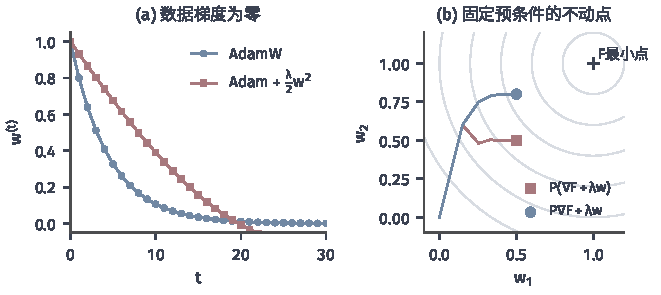
\includegraphics[width=112mm]{figures/03-optimization-evolution-and-signals/01-optimization/matplotlib/c8-decay-vs-l2/figure.pdf}
  \caption{显式二次正则与解耦衰减。(a)~数据梯度恒为零时的标量迭代，$w^{(0)}=1$，$\eta=0.1$，$\lambda=2$，$\varepsilon=1$，$\beta_1=0.9$，$\beta_2=0.999$：AdamW（圆点）每步乘$0.8$；加入$\tfrac\lambda2w^2$后的Adam（方块）首步为$14/15$，此后近似线性下降并越过零。(b)~固定预条件$\bm P=\operatorname{diag}(1,4)$下，对$F(\bm w)=\tfrac12\|\bm w-(1,1)\|_2^2$、$\lambda=1$、$\eta=0.15$从原点出发的两条轨迹：更新$\bm w-\eta\bm P(\nabla F+\lambda\bm w)$收敛到$(\tfrac12,\tfrac12)$，更新$\bm w-\eta(\bm P\nabla F+\lambda\bm w)$收敛到$(\tfrac12,\tfrac45)$。灰色圆是$F$的等值线。}
  \label{fig:opt-fit-decay-vs-l2}
\end{figure}

\paragraph{需要逐项记录的设置}
实际使用时，是否对偏置、归一化层参数施加衰减，各实现并不一致，所以要明确列出受衰减的参数。还要注意收缩系数的写法：有的实现写成$1-\eta^{(t)}\lambda$，衰减随学习率调度一起变化；有的写成与步长无关的$1-\lambda'$。在变步长下，$T$步累计的收缩因子分别是$\prod_{t}(1-\eta^{(t)}\lambda)$与$(1-\lambda')^T$，即使首步相同，后面也会分开。

\paragraph{固定预条件下的直接计算}
历史统计使上面的比较难以写成闭式。把Adam的逐坐标缩放换成固定的正定对角矩阵$\bm P$，差别就能精确算出。比较两种更新：
\[
  \text{(i)}\ \ \bm w^+=\bm w-\eta\bm P\bigl(\nabla F(\bm w)+\lambda\bm w\bigr),\qquad
  \text{(ii)}\ \ \bm w^+=\bm w-\eta\bigl(\bm P\nabla F(\bm w)+\lambda\bm w\bigr).
\]
(i)是对$F+\tfrac\lambda2\|\bm w\|_2^2$的预条件梯度步，不动点满足$\nabla F+\lambda\bm w=\bm 0$。(ii)可以改写为$\bm w-\eta\bm P\bigl(\nabla F+\lambda\bm P^{-1}\bm w\bigr)$，它是对另一个目标$F+\tfrac\lambda2\bm w^\top\bm P^{-1}\bm w$的预条件梯度步，不动点满足$\nabla F+\lambda\bm P^{-1}\bm w=\bm 0$。所以在固定预条件下，解耦衰减等价于把欧氏惩罚换成按$\bm P^{-1}$加权的惩罚：缩放大的坐标，受到的有效惩罚反而小。

取$F(\bm w)=\tfrac12\|\bm w-(1,1)^\top\|_2^2$、$\lambda=1$、$\bm P=\operatorname{diag}(1,4)$验算。(i)的不动点解$2\bm w=(1,1)^\top$，即$(\tfrac12,\tfrac12)$；(ii)的不动点逐坐标解$1\cdot(w_1-1)+w_1=0$与$4(w_2-1)+w_2=0$，得$(\tfrac12,\tfrac45)$。图~\ref{fig:opt-fit-decay-vs-l2}(b)中两条轨迹分别停在这两点。$\bm P$随历史变化时，(ii)连这样一个固定的等价目标也没有，需要单独分析。因此报告结果时应同时写明数据目标、显式正则目标和实际的更新规则，并按事先规定的评价目标比较，不能仅凭“都用了$\lambda$”认为它们求解的是同一个问题。

\section{线性表示中的拟合}
\label{sec:opt-fit-linear}

上一节的目标~\eqref{eq:opt-fit-general-objective}以函数为未知量。最直接的计算办法，是事先固定有限个基函数，只让它们的系数变化。这样函数拟合就变成有限维参数的优化：二次目标归结为一个最小二乘问题，可以直接调用线性代数中的分解与迭代求解器；稳健残差代价则可以借助逐轮构造的二次上界，变成一串加权最小二乘。

\subsection{线性基函数与二次正则化}
\label{sec:opt-fit-linear-basis}

\paragraph{设计矩阵与正则矩阵}
取$d$个基函数$\varphi_1,\dots,\varphi_d$，候选写成$f_{\bm w}=\sum_{j=1}^dw_j\varphi_j$。线性观测作用在它上面，得到
\[
  L_if_{\bm w}=\sum_{j=1}^dw_jL_i\varphi_j=(\bm X\bm w)_i,\qquad \bm X_{i,j}=L_i\varphi_j,
\]
称$\bm X\in\mathbb R^{n\times d}$为\term{设计矩阵}（design matrix），残差为$\bm X\bm w-\bm y$。点值观测时$\bm X_{i,j}=\varphi_j(x_i)$，就是熟悉的“特征矩阵”；积分观测时$\bm X_{i,j}$是基函数的积分。正则化同样由基函数算出：若$R(f)=\langle f,f\rangle$由某个内积给出，则$R(f_{\bm w})=\bm w^\top\bm R\bm w$，其中$\bm R_{j,k}=\langle\varphi_j,\varphi_k\rangle$；导数半范数$\int(f')^2$对应$\bm R_{j,k}=\int\varphi_j'\varphi_k'$，章首图中的曲率惩罚对应$\bm R_{j,k}=\int\varphi_j''\varphi_k''$。只有当基函数在相应内积下标准正交时，$\bm R$才是单位矩阵，函数范数才等于系数的欧氏范数。

\paragraph{同一数据上三种惩罚的选择}
取基$\{1,x\}$，只读到一个值$f(\tfrac12)=1$，于是$\bm X=(1,\tfrac12)$，一次函数$w_1+w_2x$中凡满足$w_1+w_2/2=1$的都插值数据。在这条直线上按三种惩罚选最小者。导数半范数$\bm R=\operatorname{diag}(0,1)$选出$w_2=0$，即常数$f=1$。$L^2$范数$\bm R=\bigl[\begin{smallmatrix}1&1/2\\1/2&1/3\end{smallmatrix}\bigr]$，由Lagrange条件，最小点与$\bm R^{-1}\bm X^\top=(1,0)^\top$成比例，也是常数$f=1$。系数欧氏范数$\bm R=\bm I$则选出与$\bm X^\top=(1,\tfrac12)^\top$成比例的点，即$\bm w=(\tfrac45,\tfrac25)$，$f(x)=\tfrac45+\tfrac25x$。三种惩罚在同一读数下给出两种不同的函数，而系数范数的选择会随基的改变而改变。

\paragraph{增广最小二乘}
设读数权重$\omega_i>0$给定，记$\bm\Omega=\operatorname{diag}(\omega_1,\dots,\omega_n)$，正则矩阵$\bm R$对称半正定，$\lambda>0$。拟合目标是
\begin{equation}
  \min_{\bm w\in\mathbb R^d}\ \frac12\bigl\|\bm\Omega^{1/2}(\bm X\bm w-\bm y)\bigr\|_2^2+\frac\lambda2\bm w^\top\bm R\bm w .
  \label{eq:opt-fit-quadratic}
\end{equation}
把$\bm R$分解为$\bm R=\bm B^\top\bm B$（例如Cholesky分解或对称平方根），惩罚就是$\tfrac\lambda2\|\bm B\bm w\|_2^2$，于是式~\eqref{eq:opt-fit-quadratic}等价于\term{增广最小二乘}（augmented least squares）
\begin{equation}
  \min_{\bm w}\ \frac12\left\|\begin{bmatrix}\bm\Omega^{1/2}\bm X\\ \sqrt\lambda\,\bm B\end{bmatrix}\bm w-\begin{bmatrix}\bm\Omega^{1/2}\bm y\\ \bm 0\end{bmatrix}\right\|_2^2,
  \label{eq:opt-fit-augmented}
\end{equation}
其正规方程为$(\bm X^\top\bm\Omega\bm X+\lambda\bm R)\bm w=\bm X^\top\bm\Omega\bm y$。$\bm R=\bm I$、$\bm\Omega=\bm I$时，这就是\term{岭回归}（ridge regression），也称\term{Tikhonov正则化}（Tikhonov regularization）。

\paragraph{唯一性由共同零方向决定}
最小二乘问题~\eqref{eq:opt-fit-augmented}的解唯一，当且仅当增广矩阵列满秩，即它的零空间只含零向量。增广矩阵作用在$\bm w$上为零，等价于$\bm\Omega^{1/2}\bm X\bm w=\bm 0$且$\bm B\bm w=\bm 0$；由$\omega_i>0$，前者即$\bm X\bm w=\bm 0$；由$\bm w^\top\bm R\bm w=\|\bm B\bm w\|_2^2$与$\bm R\succeq\bm 0$，后者即$\bm R\bm w=\bm 0$。所以
\[
  \text{式~\eqref{eq:opt-fit-quadratic}的解唯一}\iff\ker\bm X\cap\ker\bm R=\{\bm 0\}.
\]
读数看不见的方向，只要惩罚能看见，就被惩罚确定；两者都看不见的方向，目标值沿它不变，解就不唯一。上面的例子中，$\ker\bm X=\operatorname{span}\{(1,-2)^\top\}$，导数半范数的$\ker\bm R=\operatorname{span}\{(1,0)^\top\}$，两者只交于零，所以即使惩罚本身是半范数，解也唯一。

\paragraph{岭回归的谱滤波}
$\bm R=\bm I$时，借助奇异值分解可以看清正则化对每个方向做了什么。设$\bm X=\sum_{k=1}^r\sigma_k\bm u_k\bm v_k^\top$，$\sigma_k>0$。正规方程$(\bm X^\top\bm X+\lambda\bm I)\bm w=\bm X^\top\bm y$在基$\{\bm v_k\}$下逐坐标解开，得到
\begin{equation}
  \bm w_\lambda=\sum_{k=1}^r\frac{\sigma_k^2}{\sigma_k^2+\lambda}\cdot\frac{\bm u_k^\top\bm y}{\sigma_k}\,\bm v_k ,
  \label{eq:opt-fit-ridge-svd}
\end{equation}
零奇异值方向（即$\ker\bm X$）的系数为零。$\bm u_k^\top\bm y/\sigma_k$是不加正则时沿$\bm v_k$的最小二乘系数，前面的因子$\sigma_k^2/(\sigma_k^2+\lambda)$称为\term{滤波因子}（filter factor）。图~\ref{fig:opt-fit-ridge-filter}显示，它在$\sigma_k\gg\sqrt\lambda$时接近$1$，几乎不改变该方向；在$\sigma_k\ll\sqrt\lambda$时近似为$\sigma_k^2/\lambda$，把该方向压到接近零；过渡发生在$\sigma_k=\sqrt\lambda$附近，那里恰好保留一半。小奇异值方向上的最小二乘系数$\bm u_k^\top\bm y/\sigma_k$会把读数的微小变化放大$1/\sigma_k$倍，岭回归削弱的正是这些方向。

\begin{figure}[!htbp]
  \centering
  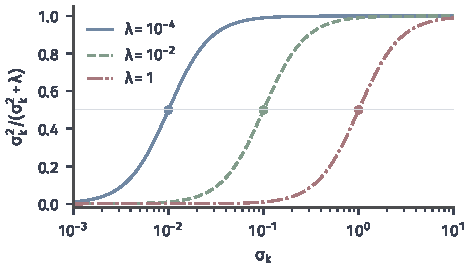
\includegraphics[width=80mm]{figures/03-optimization-evolution-and-signals/01-optimization/matplotlib/c8-ridge-filter/figure.pdf}
  \caption{岭回归在奇异值方向上的滤波因子$\sigma_k^2/(\sigma_k^2+\lambda)$，横轴为对数刻度，$\lambda=10^{-4},10^{-2},1$。圆点标出$\sigma_k=\sqrt\lambda$处因子恰为$\tfrac12$；大于$\sqrt\lambda$的奇异值方向基本保留，小于$\sqrt\lambda$的方向被压向零。}
  \label{fig:opt-fit-ridge-filter}
\end{figure}

\paragraph{求解器的选择}
式~\eqref{eq:opt-fit-augmented}是标准的线性最小二乘问题，QR分解、奇异值分解、LSQR等求解方法及伪逆与最小范数解的性质，可参考\BookChapterRef{chap:linear-equations-and-optimization}{卷一“线性方程与矩阵方程”章}；这里只说明怎样按问题结构选用。矩阵规模中等、增广矩阵列满秩时，对它做QR分解最稳妥，避免显式形成正规方程，后者会把条件数平方。要对许多个$\lambda$求解，或$\bm X$接近秩亏时，先做一次奇异值分解，再由式~\eqref{eq:opt-fit-ridge-svd}对每个$\lambda$只花$O(rd)$的代价组合系数。$\bm X$大而稀疏、只能做矩阵向量乘积时，用LSQR一类的Krylov方法直接作用于增广系统，它们原生支持“阻尼”项$\sqrt\lambda\bm I$，每轮只需一次$\bm X\bm v$与一次$\bm X^\top\bm u$。

\subsection{稳健拟合与迭代重加权最小二乘}
\label{sec:opt-fit-irls}

平方代价把远离其他读数的点看得很重。图~\ref{fig:opt-fit-irls}(a)中十四个点大致沿直线$y=1+2x$分布，其中两点被人为下移了两个多单位；普通最小二乘直线被它们拉得几乎放平，斜率只有$0.71$。换用对大残差增长较慢的代价可以减轻这种影响，但目标不再是二次的。本小节说明，对一类常用的稳健代价，可以逐轮构造一个二次上界，把问题化成一串加权最小二乘。

\paragraph{从残差平方的凹函数出发}
固定线性残差$r_i(\bm w)=\bm X_{i,:}\bm w-y_i$，把目标写成残差平方的函数
\begin{equation}
  F(\bm w)=\frac12\sum_{i=1}^n\rho\bigl(r_i(\bm w)^2\bigr),
  \label{eq:opt-fit-robust-objective}
\end{equation}
其中$\rho:[0,\infty)\to\mathbb R$可微、非减，并且对平方残差$s=r^2$是凹函数。平方代价对应$\rho(s)=s$；Huber损失对应$\rho(s)=s$（$s\le\delta^2$）与$\rho(s)=2\delta\sqrt s-\delta^2$（$s>\delta^2$）；Cauchy代价对应$\rho(s)=c^2\log(1+s/c^2)$，$c>0$为尺度。它们的导数$\rho'(r^2)$分别是$1$、$\min\{1,\delta/|r|\}$与$1/(1+r^2/c^2)$，正是图~\ref{fig:opt-fit-residual-losses}(b)中的权重曲线。绝对值代价对应$\rho(s)=2\sqrt s$，在$s=0$处不可微，权重$1/|r|$在零残差处无界，不满足这里的条件。

\paragraph{切线给出二次上界}
凹函数位于它任一点的切线之下：对$s,s_0\ge0$，$\rho(s)\le\rho(s_0)+\rho'(s_0)(s-s_0)$。在当前点$\bm w^{(t)}$处记$s_i^{(t)}=r_i(\bm w^{(t)})^2$，令\emph{权重}
\[
  \gamma_i^{(t)}=\rho'\bigl(s_i^{(t)}\bigr)\ge0,
\]
非负性来自$\rho$非减。把切线不等式用于每个$s=r_i(\bm w)^2$并求和，得到
\begin{equation}
  F(\bm w)\le Q(\bm w\mid\bm w^{(t)})
  =\frac12\sum_{i=1}^n\Bigl[\rho\bigl(s_i^{(t)}\bigr)+\gamma_i^{(t)}\bigl(r_i(\bm w)^2-s_i^{(t)}\bigr)\Bigr],
  \label{eq:opt-fit-irls-surrogate}
\end{equation}
且$\bm w=\bm w^{(t)}$时两边相等。$Q$关于$\bm w$是加权平方和加常数，所以极小化它就是解一个\term{加权最小二乘}（weighted least squares）问题。这正是第~\ref{chap:opt-nonsmooth}章主化--最小化（MM）方法的构造：代理在全域位于原目标之上、在当前点与之相切，于是对代理的任何改善都传给原目标，
\[
  F(\bm w^{(t+1)})\le Q(\bm w^{(t+1)}\mid\bm w^{(t)})\le Q(\bm w^{(t)}\mid\bm w^{(t)})=F(\bm w^{(t)}).
\]
权重必须由同一个$\rho$在当前残差处求导得到；若随意重设权重，代理就不再是$F$的上界，这条不等式链随之失效。

\begin{algorithm}[迭代重加权最小二乘]
\label{alg:opt-fit-irls}
\begin{algorithmic}[1]
\Require 设计矩阵$\bm X$、读数$\bm y$、满足上述条件的$\rho$、初值$\bm w^{(0)}$、容许误差$\epsilon>0$、最大轮数$T$
\Ensure 参数$\bm w$及其目标值$F(\bm w)$
\For{$t=0,1,\dots,T-1$}
  \State 计算残差$r_i=\bm X_{i,:}\bm w^{(t)}-y_i$与权重$\gamma_i=\rho'(r_i^2)$，记$\bm\Gamma=\operatorname{diag}(\gamma_i)$
  \State 以QR或SVD求解$\min_{\bm w}\|\bm\Gamma^{1/2}(\bm X\bm w-\bm y)\|_2^2$，得候选$\tilde{\bm w}$
  \State 若$Q(\tilde{\bm w}\mid\bm w^{(t)})>Q(\bm w^{(t)}\mid\bm w^{(t)})$，报告子问题求解失败并停止
  \State $\bm w^{(t+1)}\gets\tilde{\bm w}$
  \If{$F(\bm w^{(t)})-F(\bm w^{(t+1)})\le\epsilon\,(1+F(\bm w^{(t)}))$}
    \State \Return $\bm w^{(t+1)}$
  \EndIf
\EndFor
\State \Return $\bm w^{(T)}$
\end{algorithmic}
\end{algorithm}

算法~\ref{alg:opt-fit-irls}称为\term{迭代重加权最小二乘}（iteratively reweighted least squares，IRLS）。每轮的主要代价是一次$n\times d$的加权最小二乘，用QR分解约为$O(nd^2)$；把$\sqrt{\gamma_i}$乘到$\bm X$与$\bm y$的第$i$行上，就能直接调用普通最小二乘求解器。第4步的检查不是多余的：当子问题只被近似求解时，只有代理确实不增，上面的下降链才成立。

\begin{example}[用常数拟合$0,0,10$]
\label{ex:opt-fit-irls-cauchy}
取$\bm X=(1,1,1)^\top$，$\bm y=(0,0,10)^\top$，Cauchy代价$c=1$，即$F(w)=\tfrac12\sum_i\log(1+(w-y_i)^2)$，初值$w^{(0)}=0$。残差为$0,0,-10$，权重$\gamma_i=1/(1+r_i^2)$依次为$1,1,1/101$。加权最小二乘的解是加权平均
\[
  w^{(1)}=\frac{1\cdot0+1\cdot0+\tfrac1{101}\cdot10}{1+1+\tfrac1{101}}=\frac{10}{203}\approx0.0493 .
\]
目标值从$F(0)\approx2.3076$降到$F(w^{(1)})\approx2.3051$。重算权重后继续迭代，序列很快稳定在$w\approx0.0499$。远处的读数$10$只得到约$1/100$的权重，几乎不影响结果，这与均值$10/3$形成对照。
\end{example}

图~\ref{fig:opt-fit-irls}(b)画出了这个例子的原目标与首轮代理：黄色虚线是$w^{(0)}=0$处构造的二次函数，它处处位于蓝色曲线之上，在$w=0$处与之相切，其最小点$10/203$就是红点所示的新迭代。同一图还暴露出$F$的非凸性：在$w\approx9.79$处另有一个局部最小点，目标值约$4.59$，远高于$2.31$。若从$w^{(0)}=10$出发，权重变为$1/101,1/101,1$，IRLS会停在这个局部最小点。代理下降只保证目标不增，不保证找到非凸目标的全局最小点；初值通常取普通最小二乘解或其他稳健的粗估计。

\begin{figure}[!htbp]
  \centering
  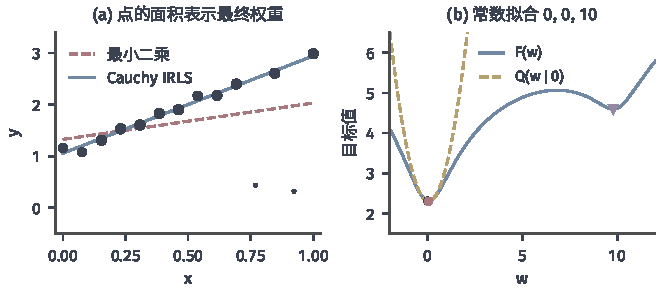
\includegraphics[width=112mm]{figures/03-optimization-evolution-and-signals/01-optimization/matplotlib/c8-irls-outliers/figure.pdf}
  \caption{稳健拟合与迭代重加权。(a)~教学示例数据：$14$个点$y=1+2x$加固定种子的小噪声，其中两点下移$2.2$与$2.6$。红色虚线为普通最小二乘直线（截距$1.33$、斜率$0.71$）；蓝线为Cauchy代价（$c=0.2$）的IRLS结果（截距$1.06$、斜率$1.89$）；点的面积正比于最终权重，两个离群点的权重约为$0.009$与$0.006$，其余点不低于$0.71$。(b)~用常数$w$拟合$0,0,10$的Cauchy目标$F(w)$（$c=1$，蓝线）与$w^{(0)}=0$处的代理$Q(w\mid0)$（黄色虚线）；黑点为初值，红点为首轮更新$10/203$，紫色三角为$w\approx9.79$处的局部最小点。}
  \label{fig:opt-fit-irls}
\end{figure}

\paragraph{权重退化、子问题误差与永久正则}
三种情形需要在实现中单独处理。第一，有些代价（例如在阈值外权重恰为零的Tukey双权代价）会给大残差零权重；若权重为零的行太多，使$\bm\Gamma^{1/2}\bm X$不再列满秩，加权最小二乘不唯一，此时应取最小范数解或检查初值与尺度，而不是任意选一个解。对绝对值代价，常用的补救是把权重改为$1/\max\{|r_i|,\epsilon\}$，但这相当于换成了一个光滑化的目标，结论要对新目标陈述。第二，子问题用迭代法近似求解时，按算法第4步检验代理值。第三，若原问题本身含正则项，例如$F(\bm w)+\tfrac\lambda2\|\bm w\|_2^2$，这一项不需要线性化，应原样加进每一轮的代理，于是每轮求解的是带同一$\lambda$的增广最小二乘~\eqref{eq:opt-fit-augmented}；它是目标的一部分，与下一节为控制步长而临时加入的阻尼不同。

\section{非线性参数的拟合}
\label{sec:opt-fit-nonlinear}

把函数写成$\sum_jw_j\varphi_j$时，读数对参数是线性的。指数衰减$\theta_1e^{-\theta_2t}$、带可学习位置的核函数、神经网络等模型则不然：候选$f_{\bm\theta}$对参数$\bm\theta\in\mathbb R^d$非线性，残差不再是$\bm\theta$的仿射函数。本节的思路是在当前点把残差或模型输出线性化，借用上一节的最小二乘机器求出候选步，再回到原目标判断这一步能不能接受。线性化只在当前点附近可信，这一点贯穿三种方法：Gauss--Newton法直接相信线性模型，Levenberg--Marquardt法用阻尼控制走出多远，广义Gauss--Newton法把同样的做法推广到一般损失。

\subsection{残差线性化与Gauss--Newton法}
\label{sec:opt-fit-gauss-newton}

\paragraph{梯度、Hessian与被省略的项}
设残差$\bm r(\bm\theta)=(r_1(\bm\theta),\dots,r_n(\bm\theta))^\top$二次连续可微，$\bm J(\bm\theta)\in\mathbb R^{n\times d}$是它的Jacobian矩阵，$\bm J_{i,:}=\nabla r_i(\bm\theta)^\top$。非线性最小二乘目标$F(\bm\theta)=\tfrac12\|\bm r(\bm\theta)\|_2^2$的梯度与Hessian由链式法则得到：
\begin{equation}
  \nabla F=\bm J^\top\bm r,\qquad
  \nabla^2F=\bm J^\top\bm J+\sum_{i=1}^nr_i\nabla^2r_i .
  \label{eq:opt-fit-nls-derivatives}
\end{equation}
第二项是各残差的二阶导数按残差大小加权求和。在当前点$\bm\theta$把残差线性化，$\bm r(\bm\theta+\bm p)\approx\bm r+\bm J\bm p$，代入目标得到线性最小二乘子问题
\begin{equation}
  \min_{\bm p\in\mathbb R^d}\ m(\bm p)=\frac12\|\bm r+\bm J\bm p\|_2^2 .
  \label{eq:opt-fit-gn-model}
\end{equation}
$m$的Hessian是$\bm J^\top\bm J$，所以\term{Gauss--Newton法}（Gauss--Newton method）相当于在牛顿法中省略式~\eqref{eq:opt-fit-nls-derivatives}的第二项。当残差小或残差近似线性时，被省略的项小，$\bm J^\top\bm J$是$\nabla^2F$的良好近似，而且它总是半正定的，计算时只需要一阶导数。

\paragraph{求步：用最小二乘而不是正规方程}
子问题~\eqref{eq:opt-fit-gn-model}的正规方程是$\bm J^\top\bm J\bm p=-\bm J^\top\bm r$，但应直接对$\bm J$做QR或奇异值分解来解。原因在于条件数：$\kappa(\bm J^\top\bm J)=\kappa(\bm J)^2$。若$\bm J$的两个奇异值为$1$与$10^{-4}$，$\kappa(\bm J)=10^4$，而正规方程的条件数为$10^8$；在双精度下，后者可能丢失约八位有效数字，前者只丢失约四位。

\paragraph{秩亏时取最小范数步并检验下降}
$\bm J$满列秩时，子问题有唯一解$\bm p=-\bm J^\dagger\bm r$。秩亏时子问题有一族解，相差$\ker\bm J$中的向量；沿这些方向线性模型不变，却不说明原目标不变。通常取其中欧氏范数最小的一个，仍记为$\bm p=-\bm J^\dagger\bm r$。这个方向是不是原目标的下降方向？直接计算方向导数：
\[
  \langle\nabla F,\bm p\rangle=-\bm r^\top\bm J\bm J^\dagger\bm r=-\|\bm J\bm J^\dagger\bm r\|_2^2 ,
\]
这里用了$\bm J\bm J^\dagger$是到$\operatorname{range}\bm J$的正交投影。由于$\operatorname{range}\bm J$与$\ker\bm J^\top$正交互补，$\bm J\bm J^\dagger\bm r=\bm 0$当且仅当$\bm J^\top\bm r=\nabla F=\bm 0$。所以只要当前点不是驻点，Gauss--Newton方向就是下降方向。下降方向只保证足够小的步长使$F$下降，单位步长未必如此，所以实际实现用原目标$F$做回溯线搜索，接受满足充分下降条件的步长；回溯规则见第~\ref{chap:opt-smooth}章。

\paragraph{局部二次收敛的条件}
在解$\bm\theta^\star$附近，若残差为零（$\bm r(\bm\theta^\star)=\bm 0$）、$\bm J(\bm\theta^\star)$满列秩、$\bm J$在$\bm\theta^\star$附近Lipschitz连续，则从足够近的初值出发、取单位步长的Gauss--Newton迭代二次收敛到$\bm\theta^\star$\scite{math-nocedal2006numerical}。一维例子可以完整验算：$r(\theta)=\theta^2-4$，零残差解$\theta^\star=2$，$J=2\theta$，Gauss--Newton步给出
\[
  \theta^+=\theta-\frac{\theta^2-4}{2\theta}=\frac{\theta^2+4}{2\theta},\qquad
  \theta^+-2=\frac{(\theta-2)^2}{2\theta}.
\]
从$\theta=3$出发，误差依次为$1$、$1/6$、$1/156\approx6.4\times10^{-3}$、约$1.0\times10^{-5}$，每步误差约为上一步的平方。

\paragraph{非零残差时被省略的项决定收敛}
残差在解处不为零时，被省略的$\bm S=\sum_ir_i\nabla^2r_i$不再消失。设$\bm\theta^\star$满足$\nabla F(\bm\theta^\star)=\bm J^\top\bm r=\bm 0$且$\bm J^\star=\bm J(\bm\theta^\star)$满列秩，把单位步长的迭代看成映射$\bm\theta\mapsto\bm\theta-(\bm J^\top\bm J)^{-1}\bm J^\top\bm r$。在$\bm\theta^\star$处求导，由于$\bm J^\top\bm r=\bm 0$，对$(\bm J^\top\bm J)^{-1}$求导的那一项消失，剩下
\[
  \bm I-(\bm J^{\star\top}\bm J^\star)^{-1}\bigl(\bm J^{\star\top}\bm J^\star+\bm S^\star\bigr)=-(\bm J^{\star\top}\bm J^\star)^{-1}\bm S^\star .
\]
这个矩阵的谱半径小于$1$时迭代在$\bm\theta^\star$附近线性收敛，速率由它决定；谱半径大于$1$时$\bm\theta^\star$对单位步长迭代是排斥的。所以残差大、残差曲率大时，Gauss--Newton可能很慢甚至不收敛。还有两种情形会破坏局部模型：$\bm J$的秩在迭代中变化，使最小范数步突然变长；子问题只被粗略求解，使所得的步连线性模型都没有充分下降。线性模型下降不能直接当作原目标下降，这正是下一小节要处理的问题。

\subsection{Levenberg--Marquardt法}
\label{sec:opt-fit-levenberg-marquardt}

\paragraph{加阻尼的子问题}
线性化只在当前点附近可信，步子越长，模型越可能失真。最简单的控制办法是惩罚步长本身，求
\begin{equation}
  \min_{\bm p}\ \frac12\|\bm r+\bm J\bm p\|_2^2+\frac\tau2\|\bm p\|_2^2,
  \qquad\text{即}\qquad
  (\bm J^\top\bm J+\tau\bm I)\bm p=-\bm J^\top\bm r ,
  \label{eq:opt-fit-lm-step}
\end{equation}
其中$\tau>0$是阻尼参数（本章用$\tau$，以免与正则化参数$\lambda$、核积分算子的特征值$\mu_j$混淆）。这就是\term{Levenberg--Marquardt法}（Levenberg--Marquardt method）的求步方程。$\tau>0$使系数矩阵正定，即使$\bm J$秩亏，步长也唯一。与第~\ref{sec:opt-fit-linear-basis}小节一样，它可以写成增广最小二乘$\min_{\bm p}\tfrac12\bigl\|\bigl[\begin{smallmatrix}\bm J\\\sqrt\tau\bm I\end{smallmatrix}\bigr]\bm p+\bigl[\begin{smallmatrix}\bm r\\\bm 0\end{smallmatrix}\bigr]\bigr\|_2^2$，用QR或LSQR求解；迭代求解时以线性系统的残差控制精度。

阻尼与正则化外形相似，作用不同。正则项$\tfrac\lambda2\|\bm\theta\|^2$永久改变目标及其最小点；阻尼$\tfrac\tau2\|\bm p\|^2$只惩罚本轮位移，在驻点处$\nabla F=\bm 0$使$\bm p=\bm 0$，不改变原目标的任何驻点。

\paragraph{阻尼在Gauss--Newton步与梯度方向之间插值}
用$\bm J$的奇异值分解$\bm J=\sum_k\sigma_k\bm u_k\bm v_k^\top$可以看清$\tau$的作用：
\[
  \bm p(\tau)=-\sum_k\frac{\sigma_k}{\sigma_k^2+\tau}(\bm u_k^\top\bm r)\bm v_k,\qquad
  \|\bm p(\tau)\|_2^2=\sum_k\frac{\sigma_k^2(\bm u_k^\top\bm r)^2}{(\sigma_k^2+\tau)^2}.
\]
由此读出三点。$\tau\downarrow0$时，系数趋于$1/\sigma_k$，$\bm p(\tau)\to-\bm J^\dagger\bm r$，即最小范数Gauss--Newton步。$\tau\to\infty$时，$\tau\bm p(\tau)\to-\sum_k\sigma_k(\bm u_k^\top\bm r)\bm v_k=-\bm J^\top\bm r=-\nabla F$，步子变短并转向负梯度方向。步长$\|\bm p(\tau)\|_2$随$\tau$单调递减。图~\ref{fig:opt-fit-lm-path}在一个两参数指数拟合问题上画出了整条路径$\bm\theta^{(0)}+\bm p(\tau)$：它从靠近最小点的Gauss--Newton点出发，随$\tau$增大缩回到起点附近，并在起点处与负梯度相切。大阻尼给出保守的梯度步，小阻尼给出大胆的模型步，$\tau$在两者之间连续调节。

\begin{figure}[!htbp]
  \centering
  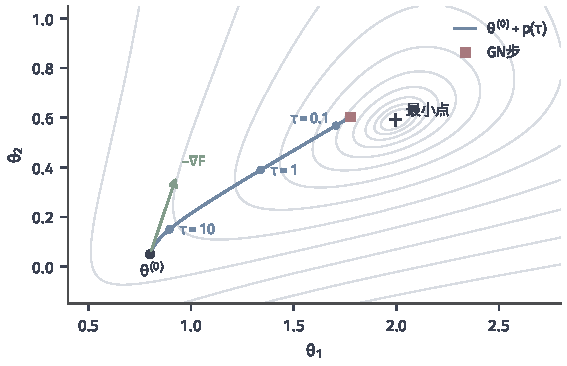
\includegraphics[width=96mm]{figures/03-optimization-evolution-and-signals/01-optimization/matplotlib/c8-lm-path/figure.pdf}
  \caption{Levenberg--Marquardt步随阻尼的变化。拟合模型$\theta_1e^{-\theta_2t}$到读数$t=0,\dots,4$，$y=(2.0,1.1,0.6,0.35,0.2)$；灰线为$\log_{10}F$的等值线，十字为最小点$(2.00,0.59)$。从$\bm\theta^{(0)}=(0.8,0.05)$出发，蓝线是$\tau$从$0$到$\infty$时的候选点$\bm\theta^{(0)}+\bm p(\tau)$，方块为$\tau=0$的Gauss--Newton点$(1.78,0.60)$，圆点标出$\tau=0.1,1,10$；绿色箭头为负梯度方向，大阻尼的步沿它离开起点。}
  \label{fig:opt-fit-lm-path}
\end{figure}

\paragraph{预报下降与接受检验}
候选步由模型算出，是否接受要回到原目标判断。用未加阻尼的线性模型$m(\bm p)=\tfrac12\|\bm r+\bm J\bm p\|_2^2$计算\term{预报下降}（predicted reduction）$\operatorname{pred}=m(\bm 0)-m(\bm p)$，与实际下降$\operatorname{ared}=F(\bm\theta)-F(\bm\theta+\bm p)$比较，比值
\begin{equation}
  \varrho=\frac{\operatorname{ared}}{\operatorname{pred}}
  \label{eq:opt-fit-lm-ratio}
\end{equation}
接近$1$说明模型可信，接近零或为负说明模型在这一步失真。式~\eqref{eq:opt-fit-lm-step}被精确求解时，预报下降总为正：由$\bm J^\top\bm r=-(\bm J^\top\bm J+\tau\bm I)\bm p$，
\[
  \operatorname{pred}=-\bm r^\top\bm J\bm p-\frac12\|\bm J\bm p\|_2^2
  =\bm p^\top(\bm J^\top\bm J+\tau\bm I)\bm p-\frac12\|\bm J\bm p\|_2^2
  =\frac12\|\bm J\bm p\|_2^2+\tau\|\bm p\|_2^2 ,
\]
它在$\bm p\ne\bm 0$（即$\nabla F\ne\bm 0$）时严格为正。因此若算出的预报下降不为正，应先检查求步是否足够精确或导数是否有误；若梯度已为零，则报告驻点并检查其性质。这里的比值检验与第~\ref{chap:opt-smooth}章信赖域方法的接受规则同源，阻尼$\tau$与信赖域半径扮演对偶的角色。

\begin{algorithm}[Levenberg--Marquardt法]
\label{alg:opt-fit-lm}
\begin{algorithmic}[1]
\Require 残差$\bm r$及其Jacobian、初值$\bm\theta^{(0)}$、初始阻尼$\tau^{(0)}>0$、接受阈值$0<\eta_a<\tfrac14$、梯度容许误差$\epsilon$
\Ensure 参数$\bm\theta$
\For{$t=0,1,2,\dots$}
  \State 计算$\bm r$、$\bm J$与$\nabla F=\bm J^\top\bm r$；若$\|\nabla F\|_2\le\epsilon$，返回$\bm\theta^{(t)}$
  \State 以增广最小二乘解式~\eqref{eq:opt-fit-lm-step}得$\bm p$，计算$\operatorname{pred}$与$\varrho$
  \If{$\varrho>\eta_a$}
    \State $\bm\theta^{(t+1)}\gets\bm\theta^{(t)}+\bm p$ \Comment{接受}
  \Else
    \State $\bm\theta^{(t+1)}\gets\bm\theta^{(t)}$ \Comment{拒绝}
  \EndIf
  \State 若$\varrho<\tfrac14$则$\tau^{(t+1)}\gets4\tau^{(t)}$；若$\varrho>\tfrac34$则$\tau^{(t+1)}\gets\tau^{(t)}/2$；否则不变
\EndFor
\end{algorithmic}
\end{algorithm}

每轮的主要代价是一次Jacobian计算与一次$(n+d)\times d$增广最小二乘求解；被拒绝的轮次只增大阻尼，不重新计算Jacobian。

\begin{example}[阻尼挽救一次发散的步]
\label{ex:opt-fit-lm-scalar}
取$r(\theta)=\theta^2-4$，$\theta^{(0)}=\tfrac12$，则$r=-\tfrac{15}4$，$J=1$，$F(\theta^{(0)})=\tfrac12\cdot\tfrac{225}{16}=\tfrac{225}{32}\approx7.03$。无阻尼时$p=-r/J=\tfrac{15}4$，新点$\theta=\tfrac{17}4$处$r=\tfrac{225}{16}$，$F=\tfrac{50625}{512}\approx98.9$，目标反而增大十几倍。取$\tau=4$，$p=-Jr/(J^2+\tau)=\tfrac{15/4}{5}=\tfrac34$，新点$\theta=\tfrac54$处$r=-\tfrac{39}{16}$，$F=\tfrac{1521}{512}\approx2.97$。预报下降为$\tfrac12(Jp)^2+\tau p^2=\tfrac9{32}+\tfrac{72}{32}=\tfrac{81}{32}$，实际下降为$\tfrac{225}{32}-\tfrac{1521}{512}=\tfrac{2079}{512}$，比值$\varrho=\tfrac{77}{48}\approx1.60>\tfrac34$，于是接受这一步，并把阻尼减半为$2$。
\end{example}

图~\ref{fig:opt-fit-gn-lm-scalar}把这个例子画了出来。黄色虚线是在$\theta^{(0)}$处线性化残差得到的模型$m$，它是一条开口向上、最小点远在$\theta=\tfrac{17}4$的抛物线，而原目标$F$在$\theta=2$之后迅速上升；Gauss--Newton步完全相信这条抛物线，跳过了真正的最小点。加阻尼后的模型（绿色点划线）在起点附近更陡地弯起，最小点被拉回到$\theta=\tfrac54$，这一步落在$F$确实下降的区域。阻尼控制的是线性化误差，而不只是让方程可逆：本例中$J=1$本来就可逆。

\begin{figure}[!htbp]
  \centering
  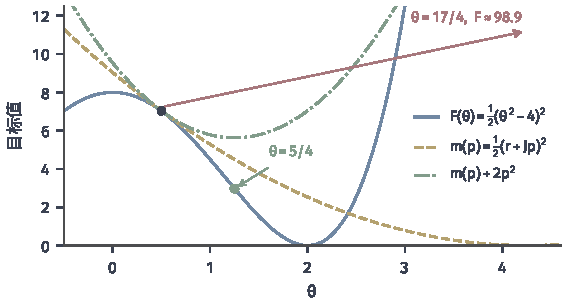
\includegraphics[width=96mm]{figures/03-optimization-evolution-and-signals/01-optimization/matplotlib/c8-gn-lm-scalar/figure.pdf}
  \caption{一维非线性最小二乘$F(\theta)=\tfrac12(\theta^2-4)^2$上的Gauss--Newton步与Levenberg--Marquardt步。蓝线为原目标，黑点为$\theta^{(0)}=\tfrac12$；黄色虚线为线性化模型$m(p)=\tfrac12(r+Jp)^2$，其最小点$\theta=\tfrac{17}4$处原目标约为$98.9$（红色箭头）；绿色点划线为加阻尼$\tau=4$的模型$m(p)+2p^2$，其最小点$\theta=\tfrac54$处原目标降到约$2.97$（绿点）。}
  \label{fig:opt-fit-gn-lm-scalar}
\end{figure}

\paragraph{条件与局限}
Levenberg--Marquardt法在每轮子问题上都有唯一解，配合比值检验能保证接受的步使原目标下降。但这不意味着找到全局最小点：非凸的$F$可能有多个局部最小点，算法停在哪一个取决于初值；收敛速率也没有统一的结论，在零残差且Jacobian满列秩的解附近，阻尼趋于零时它表现得像Gauss--Newton法，否则可能只有线性速率。若把它用作非线性残差IRLS的内层求解器，每轮要检查的是完整的加权代理~\eqref{eq:opt-fit-irls-surrogate}是否下降，而不只是检查一次线性化模型。

\subsection{一般损失与广义Gauss--Newton法}
\label{sec:opt-fit-ggn}

平方损失只是一种选择。分类模型常用交叉熵，稳健回归用Huber损失，模型的输出也可能是向量。本小节把Gauss--Newton的思路推广到一般损失：仍然把模型输出线性化，但对损失保留完整的二阶信息。

\paragraph{链式法则分出两类二阶项}
设第$i$个样本的模型输出为$\bm h_i(\bm\theta)\in\mathbb R^{q}$，损失为$\ell_i(\bm z)$，目标为$F(\bm\theta)=\frac1n\sum_{i=1}^n\ell_i(\bm h_i(\bm\theta))$。在当前点记输出Jacobian $\bm J_i=D\bm h_i(\bm\theta)\in\mathbb R^{q\times d}$、损失对输出的梯度$\bm a_i=\nabla\ell_i(\bm h_i)$与Hessian $\bm S_i=\nabla^2\ell_i(\bm h_i)$。链式法则给出
\[
  \nabla F=\frac1n\sum_i\bm J_i^\top\bm a_i,\qquad
  \nabla^2F=\frac1n\sum_i\Bigl[\bm J_i^\top\bm S_i\bm J_i+\sum_{k=1}^qa_{i,k}\nabla^2h_{i,k}\Bigr].
\]
第一项来自损失的曲率，第二项来自输出映射的曲率、按损失梯度加权。保留第一项、省略第二项，得到\term{广义Gauss--Newton矩阵}（generalized Gauss--Newton matrix）
\begin{equation}
  \bm H_{\mathrm{GN}}=\frac1n\sum_{i=1}^n\bm J_i^\top\bm S_i\bm J_i .
  \label{eq:opt-fit-ggn}
\end{equation}
平方损失$\ell_i(\bm z)=\tfrac12\|\bm z-\bm y_i\|_2^2$时$\bm S_i=\bm I$，它退回普通Gauss--Newton矩阵（相差因子$1/n$）。若每个$\ell_i$对输出凸且二次可微，则$\bm S_i\succeq\bm0$，从而$\bm H_{\mathrm{GN}}\succeq\bm0$。这只说明线性化后的模型是凸二次函数，复合目标$F$对参数仍可能非凸。

\paragraph{半正定不能认证没有负曲率}
一个标量例子说明两者的差距。取$n=1$，$h(\theta)=\theta^2$，$\ell(z)=\tfrac12(z-1)^2$，则$F(\theta)=\tfrac12(\theta^2-1)^2$。这里$J=2\theta$，$S=1$，$a=\theta^2-1$，$h''=2$，所以
\[
  \nabla^2F=4\theta^2+2(\theta^2-1)=6\theta^2-2,\qquad H_{\mathrm{GN}}=4\theta^2 .
\]
在$\theta=0.3$处，$H_{\mathrm{GN}}=0.36>0$，而真实曲率$\nabla^2F=-1.46<0$。广义Gauss--Newton矩阵总是半正定的，所以它不能用来认证一个驻点是局部最小点。输出映射是仿射函数时第二项为零，$\bm H_{\mathrm{GN}}=\nabla^2F$，这是舍项消失的充分条件；一般情形下，被舍去的项要另行估计。

\paragraph{矩阵自由求步}
参数很多时不能存储$d\times d$的$\bm H_{\mathrm{GN}}$，但可以计算它与任意向量$\bm v$的乘积：依次算输出方向导数$\bm J_i\bm v$、乘以损失曲率$\bm S_i(\bm J_i\bm v)$、再由反向传播得到$\bm J_i^\top(\bm S_i\bm J_i\bm v)$，对样本平均即得$\bm H_{\mathrm{GN}}\bm v$，代价约为两次前向与一次反向计算。求步方程
\[
  (\bm H_{\mathrm{GN}}+\tau\bm I)\bm p=-\nabla F
\]
在$\tau>0$与上述凸性条件下系数矩阵正定，可以用第~\ref{chap:opt-smooth}章的共轭梯度法（CG）求解，只调用矩阵向量积，并以相对残差控制内层精度。

从零初值出发的CG有一个有用的性质：每个中间近似解都是原目标的下降方向。记$\bm A=\bm H_{\mathrm{GN}}+\tau\bm I\succ\bm0$，$\bm g=\nabla F\ne\bm0$。CG的第$k$个近似$\bm p_k$在含$\bm g$的Krylov子空间中极小化$q(\bm p)=\tfrac12\bm p^\top\bm A\bm p+\bm g^\top\bm p$，于是$q(\bm p_k)\le q(-\alpha\bm g)<0$对足够小的$\alpha>0$成立，从而$\bm g^\top\bm p_k<-\tfrac12\bm p_k^\top\bm A\bm p_k<0$。因此即使提前停止CG，所得方向也能下降。接受与否仍用原目标判断：用真梯度检查$\langle\nabla F,\bm p\rangle<0$，再沿$\bm p$回溯，或像Levenberg--Marquardt法那样计算比值并调节$\tau$。

\section{Hilbert空间中的有限观测拟合}
\label{sec:opt-fit-hilbert}

前两节先固定了有限个基函数，再求系数。基函数选多少、选哪些，本身就是一个限制：真正好的函数可能不在它们张成的空间里。现在反过来，让候选取遍一个无限维Hilbert空间$H$，只保留读数是有限个这一事实。本节说明，在这一设定下，有限个读数会自动把搜索压缩到一个有限维子空间；所得的有限维问题可以用Gram矩阵写出，并在正则化与精确插值两种任务下讨论解的存在与唯一。

\subsection{正交分解与表示定理}
\label{sec:opt-fit-representer}

\paragraph{读数只看见有限个方向}
设$H$是实Hilbert空间，$L_1,\dots,L_n$是$H$上的有界线性泛函。由Riesz表示定理，每个$L_i$对应唯一的$h_i\in H$，使$L_if=\langle f,h_i\rangle_H$对一切$f\in H$成立；有界线性泛函与Riesz表示的一般理论可参考\BookChapterRef{chap:linear-functionals-operators}{卷二“线性泛函与线性算子”章}。在再生核Hilbert空间中读点值$f(x_i)$时，表示元就是核截面$h_i=K(\cdot,x_i)$；对有界连续核与有限测度$\nu$读积分$\int f\varphi_i\,\mathrm d\nu$（$\varphi_i\in L^2(\nu)$）时，表示元是$h_i=\int K(\cdot,x)\varphi_i(x)\,\mathrm d\nu(x)$，它一般不是任何一个核截面。

令$M=\operatorname{span}\{h_1,\dots,h_n\}$。它是有限维子空间，因而是闭的，到它的正交投影$P_M$存在；Hilbert空间中闭子空间的投影定理可参考\BookChapterRef{chap:function-spaces}{卷二“函数空间”章}。把任一$f\in H$分解为
\[
  f=P_Mf+r,\qquad r\perp M .
\]
余项$r$与每个$h_i$正交，所以$L_ir=\langle r,h_i\rangle=0$，即$Lf=L(P_Mf)$：去掉余项，读数一个也不变。同时由勾股定理$\|f\|_H^2=\|P_Mf\|_H^2+\|r\|_H^2\ge\|P_Mf\|_H^2$，投影不增大范数，且仅当$r=0$时范数不变。图~\ref{fig:opt-fit-representer-geometry}把这件事画成平面图：与$f$读数相同的候选组成一条与$M$垂直的直线，它与$M$的交点$P_Mf$是这条直线上离原点最近的点。

\begin{figure}[!htbp]
  \centering
  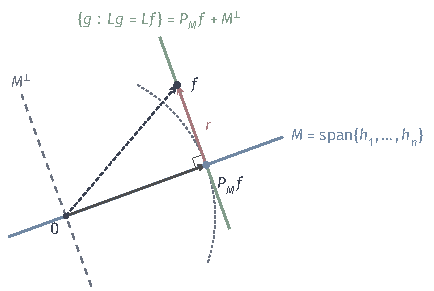
\includegraphics[width=73.5mm]{figures/03-optimization-evolution-and-signals/01-optimization/tikz/c8-representer-geometry/figure.pdf}
  \caption{表示定理的几何。蓝线为观测表示元张成的子空间$M$，灰色虚线为其正交补$M^\perp$；与$f$读数相同的全部候选组成仿射集$P_Mf+M^\perp$（绿线）。余项$r=f-P_Mf$垂直于$M$，不改变任何读数；以原点为心、过$P_Mf$的圆弧（灰色点线）与绿线相切，说明$P_Mf$是该仿射集中范数最小的元素。}
  \label{fig:opt-fit-representer-geometry}
\end{figure}

\paragraph{表示定理}
考虑一般的正则化拟合目标
\begin{equation}
  \min_{f\in H}\ J(f)=\Phi(Lf)+\Omega\bigl(\|f\|_H\bigr),
  \label{eq:opt-fit-representer-problem}
\end{equation}
其中$\Phi:\mathbb R^n\to\mathbb R\cup\{+\infty\}$是任意的数据代价（数据$\bm y$已含在$\Phi$中），$\Omega:[0,\infty)\to\mathbb R$单调不减。上面的两条观察直接给出$J(P_Mf)\le J(f)$：数据项不变，正则项不增。

\begin{theorem}[表示定理]
\label{thm:opt-fit-representer}
在上述设定下：
\begin{enumerate}
  \item $\inf_{f\in H}J(f)=\inf_{f\in M}J(f)$；
  \item 若$J$在某个$f^\star\in H$处达到最小值，则$P_Mf^\star\in M$也是最小点；
  \item 若$\Omega$严格递增，且最小值有限，则每个最小点都属于$M$，即都形如$\sum_{j=1}^na_jh_j$。
\end{enumerate}
\end{theorem}

\begin{proof}
(1) $M\subseteq H$给出$\inf_HJ\le\inf_MJ$。反过来，对任意$f\in H$，$P_Mf\in M$且$J(P_Mf)\le J(f)$，所以$\inf_MJ\le J(f)$，对$f$取下确界得$\inf_MJ\le\inf_HJ$。

(2) $J(P_Mf^\star)\le J(f^\star)=\min_HJ$，而$P_Mf^\star\in H$，所以等号成立。

(3) 设$f^\star$是最小点而$r=f^\star-P_Mf^\star\ne0$。则$\|P_Mf^\star\|_H<\|f^\star\|_H$，$\Omega$严格递增给出$\Omega(\|P_Mf^\star\|)<\Omega(\|f^\star\|)$，数据项相同，于是$J(P_Mf^\star)<J(f^\star)$，与$f^\star$是最小点矛盾（这里用到$J(f^\star)$有限）。
\end{proof}

这一结论称为\term{表示定理}（representer theorem）\scite{scholkopf2001representer}。它把一个无限维的搜索化成了$n$个系数$a_1,\dots,a_n$的搜索，代价是要知道表示元$h_i$及它们的内积。

\paragraph{定理没有说的事}
定理的三条结论都是有条件的。第1条只比较下确界，没有说最小值能达到；第2条在“若达到”的前提下才给出$M$中的最小点；第3条在$\Omega$只是单调不减（例如在某段上为常数）时可能不成立，此时$M$外也可以有最小点。最小点是否存在、是否唯一，要像下一小节那样另外证明。

候选集合另加约束时，还要检查投影是否保持可行。若约束只涉及同一组读数，例如$L_1f\ge0$，那么$P_Mf$与$f$读数相同，可行性不变。若约束涉及$M$以外的信息，结论可能失效。在$[0,1]$上以最小值核$K(s,t)=\min(s,t)$生成的空间$H_{\min}$中（其范数为$\|f\|_H^2=\int_0^1(f')^2\,\mathrm dx$，要求$f(0)=0$），只读一个点值$f(\tfrac12)=0$，于是$M=\operatorname{span}\{\min(\cdot,\tfrac12)\}$；若再要求$f(\tfrac14)\ge1$，任何可行的$f$投影后都变成$P_Mf=c\min(\cdot,\tfrac12)$，由$c/2=f(\tfrac12)=0$得$P_Mf=0$，不再满足$f(\tfrac14)\ge1$。此时最优解不必落在$M$中，约束$f(\tfrac14)\ge1$本身也是一个读数，应把它的表示元加进$M$。

\subsection{Gram矩阵与正则化平方拟合}
\label{sec:opt-fit-gram}

\paragraph{有限维问题的系数形式}
在$M$中写$f=\sum_{j=1}^na_jh_j$，$\bm a\in\mathbb R^n$。记\term{Gram矩阵}（Gram matrix）$\bm G_{i,j}=\langle h_i,h_j\rangle_H=L_ih_j$，它对称半正定。读数与范数都由它算出：
\begin{equation}
  L_if=\sum_ja_j\langle h_j,h_i\rangle=(\bm G\bm a)_i,\qquad
  \|f\|_H^2=\sum_{i,j}a_ia_j\langle h_i,h_j\rangle=\bm a^\top\bm G\bm a .
  \label{eq:opt-fit-gram-calculus}
\end{equation}
读点值时$\bm G_{i,j}=K(x_i,x_j)$，就是\term{核矩阵}（kernel matrix）；读积分等一般观测时，$\bm G$仍是表示元的Gram矩阵，但不再是核在观测点上的取值。

现在取平方数据代价与平方范数正则，$\lambda>0$：
\begin{equation}
  J(f)=\frac1n\|Lf-\bm y\|_2^2+\lambda\|f\|_H^2 .
  \label{eq:opt-fit-kernel-ridge}
\end{equation}
点值观测下，这就是\term{核岭回归}（kernel ridge regression）。由式~\eqref{eq:opt-fit-gram-calculus}，它在$M$上的系数形式是
\[
  J(\bm a)=\frac1n\|\bm G\bm a-\bm y\|_2^2+\lambda\,\bm a^\top\bm G\bm a ,\qquad
  \nabla J(\bm a)=\frac2n\bm G\bigl[(\bm G+n\lambda\bm I)\bm a-\bm y\bigr].
\]
梯度为零的条件是
\begin{equation}
  \bm G\bigl[(\bm G+n\lambda\bm I)\bm a-\bm y\bigr]=\bm 0 .
  \label{eq:opt-fit-kernel-stationary}
\end{equation}
$\bm G+n\lambda\bm I$对称正定，所以$\bm a_\lambda=(\bm G+n\lambda\bm I)^{-1}\bm y$满足它。称这个解为规范代表，它满足的方程$(\bm G+n\lambda\bm I)\bm a=\bm y$比式~\eqref{eq:opt-fit-kernel-stationary}更强。

\begin{theorem}[正则化平方拟合的解]
\label{thm:opt-fit-kernel-ridge}
设$L_i$有界，$\lambda>0$。则目标~\eqref{eq:opt-fit-kernel-ridge}在$H$上有唯一的最小点
\[
  f_\lambda=\sum_{j=1}^n(a_\lambda)_jh_j,\qquad \bm a_\lambda=(\bm G+n\lambda\bm I)^{-1}\bm y .
\]
满足式~\eqref{eq:opt-fit-kernel-stationary}的任一系数向量都给出同一个函数$f_\lambda$。
\end{theorem}

\begin{proof}
$J(\bm a)$是$\bm a$的凸二次函数（Hessian为$\tfrac2n\bm G^2+2\lambda\bm G\succeq\bm0$），所以满足式~\eqref{eq:opt-fit-kernel-stationary}的点都是它在$\mathbb R^n$上的最小点；$\bm a_\lambda$是其中之一，于是$f_\lambda$在$M$上达到最小。由表示定理第1条，$f_\lambda$也是$H$上的最小点。$\Omega(t)=\lambda t^2$在$[0,\infty)$上严格递增，由第3条，$H$上的每个最小点都在$M$中，形如$\sum_ja_jh_j$，其系数是$J(\bm a)$的最小点，因而满足式~\eqref{eq:opt-fit-kernel-stationary}。

剩下证明满足式~\eqref{eq:opt-fit-kernel-stationary}的两个系数$\bm a,\bm a'$给出同一函数。令$\bm d=\bm a-\bm a'$，相减得$\bm G(\bm G+n\lambda\bm I)\bm d=\bm 0$。左乘$\bm d^\top$，得$\|\bm G\bm d\|_2^2+n\lambda\,\bm d^\top\bm G\bm d=0$；两项都非负，故$\bm d^\top\bm G\bm d=0$。由式~\eqref{eq:opt-fit-gram-calculus}，这正是$\bigl\|\sum_jd_jh_j\bigr\|_H^2=0$，两组系数代表同一个函数。
\end{proof}

\paragraph{函数唯一不等于系数唯一}
定理中唯一的是函数，不是系数。$\bm G$奇异时，系数可以沿$\ker\bm G$任意移动而函数不变：若$\bm G\bm d=\bm 0$，则$\|\sum_jd_jh_j\|^2=\bm d^\top\bm G\bm d=0$。例如在$[-1,1]$上取仿射核$K(s,t)=1+st$，读三个点值$x=-1,0,1$，核截面$1-x$、$1$、$1+x$线性相关，$\bm G=\bigl[\begin{smallmatrix}2&1&0\\1&1&1\\0&1&2\end{smallmatrix}\bigr]$，$\ker\bm G=\operatorname{span}\{(1,-2,1)^\top\}$，对应的函数组合$(1-x)-2+(1+x)$恒为零。规范代表$\bm a_\lambda$是满足更强方程的那一个；其他满足式~\eqref{eq:opt-fit-kernel-stationary}的系数都与它相差$\ker\bm G$中的向量。数值上应以Cholesky分解求解$(\bm G+n\lambda\bm I)\bm a=\bm y$，而不显式求逆；后者多花计算，也放大舍入误差。

\begin{example}[最小值核上的两点拟合]
\label{ex:opt-fit-min-kernel}
在$H_{\min}$中读$f(\tfrac12)=1$、$f(1)=1$，$n=2$。核截面$K_{1/2}=\min(\cdot,\tfrac12)$与$K_1=\min(\cdot,1)$都是从原点出发的折线，Gram矩阵$\bm G=\bigl[\begin{smallmatrix}1/2&1/2\\1/2&1\end{smallmatrix}\bigr]$。取$\lambda=\tfrac14$，$n\lambda=\tfrac12$，
\[
  \bm G+\tfrac12\bm I=\begin{bmatrix}1&1/2\\1/2&3/2\end{bmatrix},\qquad
  \bm a_\lambda=\frac45\begin{bmatrix}3/2&-1/2\\-1/2&1\end{bmatrix}\begin{bmatrix}1\\1\end{bmatrix}=\begin{bmatrix}4/5\\2/5\end{bmatrix}.
\]
拟合函数$f_\lambda=\tfrac45\min(\cdot,\tfrac12)+\tfrac25\min(\cdot,1)$在$[0,\tfrac12]$上斜率为$\tfrac65$，在$[\tfrac12,1]$上斜率为$\tfrac25$。读数$\bm G\bm a_\lambda=(\tfrac35,\tfrac45)^\top$，都比数据$1$小；范数平方$\bm a_\lambda^\top\bm G\bm a_\lambda=\tfrac45$。图~\ref{fig:opt-fit-min-kernel}(a)画出了两条核截面（灰色点线）及其组合（蓝线）：正则化让函数以较小的范数为代价，在读数上作了让步。
\end{example}

\subsection{最小范数插值}
\label{sec:opt-fit-min-norm-interpolation}

把正则化拟合换成必须精确满足读数的任务：
\[
  \min_{f\in H}\ \|f\|_H\qquad\text{s.t.}\quad Lf=\bm y .
\]
它的解称为\term{最小范数插值}（minimum-norm interpolation）。首先要判断约束是否可满足。由$Lf=L(P_Mf)$及式~\eqref{eq:opt-fit-gram-calculus}，$L$的像集等于$\{\bm G\bm a:\bm a\in\mathbb R^n\}=\operatorname{range}\bm G$，所以插值有解当且仅当$\bm y\in\operatorname{range}\bm G$。读数不相容时问题没有可行点；此时求$\min_f\|Lf-\bm y\|$得到的是最小二乘拟合，它的残差不为零，不能当作插值。

\begin{theorem}[最小范数插值]
\label{thm:opt-fit-min-norm-interpolation}
设$\bm y\in\operatorname{range}\bm G$，令$\bm a^\dagger=\bm G^\dagger\bm y$、$f^\dagger=\sum_ja^\dagger_jh_j$。则$f^\dagger$插值数据，并且是唯一的最小范数插值函数，$\|f^\dagger\|_H^2=\bm y^\top\bm G^\dagger\bm y$。任一满足$\bm G\bm a=\bm y$的系数都给出同一函数$f^\dagger$。
\end{theorem}

\begin{proof}
$\bm G\bm G^\dagger$是到$\operatorname{range}\bm G$的正交投影，$\bm y$在其中，所以$Lf^\dagger=\bm G\bm a^\dagger=\bm y$。若$g\in H$也满足$Lg=\bm y$，则$\langle g-f^\dagger,h_i\rangle=L_i(g-f^\dagger)=0$对每个$i$成立，即$g-f^\dagger\perp M$；而$f^\dagger\in M$，由勾股定理$\|g\|_H^2=\|f^\dagger\|_H^2+\|g-f^\dagger\|_H^2\ge\|f^\dagger\|_H^2$，等号当且仅当$g=f^\dagger$。范数由$\bm a^{\dagger\top}\bm G\bm a^\dagger=\bm y^\top\bm G^\dagger\bm G\bm G^\dagger\bm y=\bm y^\top\bm G^\dagger\bm y$得到。最后，若$\bm G\bm a=\bm y=\bm G\bm a^\dagger$，则$\bm G(\bm a-\bm a^\dagger)=\bm 0$，上一小节已说明这样的两组系数给出同一函数。
\end{proof}

伪逆在系数层面选出欧氏长度最小的一组系数，但定理中的“最小范数”指函数的$H$范数，与选哪组系数无关。对点值观测，这与卷二“再生核Hilbert空间”章中观测投影的最小范数性质一致。

继续例~\ref{ex:opt-fit-min-kernel}。$\bm G$可逆，$\bm a^\dagger=\bm G^{-1}\bm y=4\bigl[\begin{smallmatrix}1&-1/2\\-1/2&1/2\end{smallmatrix}\bigr](1,1)^\top=(2,0)^\top$，于是$f^\dagger=2\min(\cdot,\tfrac12)$：从原点以斜率$2$升到$(\tfrac12,1)$，之后保持水平，$\|f^\dagger\|_H^2=\int_0^{1/2}4\,\mathrm dx=2$。另取$r(x)=\tfrac14\sin2\pi x$，它满足$r(0)=r(\tfrac12)=r(1)=0$，因而$r\perp M$，$f^\dagger+r$也插值数据，范数平方却是$2+\int_0^1(\tfrac\pi2\cos2\pi x)^2\,\mathrm dx=2+\tfrac{\pi^2}8\approx3.23$。图~\ref{fig:opt-fit-min-kernel}(b)画出这两个读数相同的插值函数：多出来的波动不被读数察觉，只增加范数。比较(a)中的红色虚线，正则化解$f_\lambda$在$\lambda\downarrow0$时趋于$f^\dagger$，第~\ref{sec:opt-fit-lambda}小节会证明这一点。

再看仿射核的例子，$\operatorname{range}\bm G=\{(1,-2,1)^\top\}^\perp$。读数$\bm y=(0,0,1)^\top$与$(1,-2,1)^\top$的内积为$1$，不在像集中：三个点不共线，仿射函数无法插值。读数$\bm y=(-1,0,1)^\top$相容，$\bm a^\dagger=(-\tfrac12,0,\tfrac12)^\top$（可验证$\bm G\bm a^\dagger=\bm y$且$\bm a^\dagger\perp(1,-2,1)^\top$），对应$f^\dagger(x)=-\tfrac12(1-x)+\tfrac12(1+x)=x$；系数$\bm a^\dagger+c(1,-2,1)^\top$给出同一个函数。

\begin{figure}[!htbp]
  \centering
  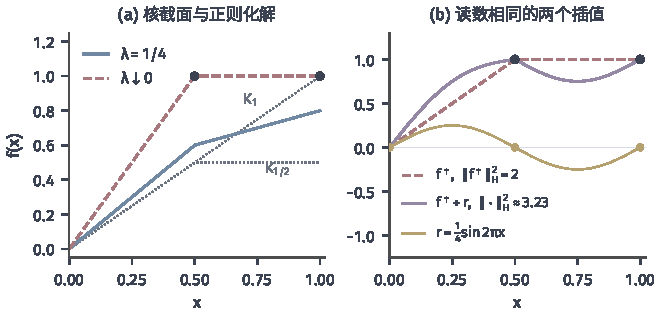
\includegraphics[width=112mm]{figures/03-optimization-evolution-and-signals/01-optimization/matplotlib/c8-min-kernel-fit/figure.pdf}
  \caption{最小值核$K(s,t)=\min(s,t)$空间中读$f(\tfrac12)=f(1)=1$（黑点）。(a)~灰色点线为核截面$K_{1/2}$与$K_1$；蓝线为$\lambda=\tfrac14$的正则化解$f_\lambda=\tfrac45K_{1/2}+\tfrac25K_1$，读数为$\tfrac35,\tfrac45$；红色虚线为$\lambda\downarrow0$的极限，即最小范数插值$f^\dagger=2K_{1/2}$。(b)~$f^\dagger$与另一个插值$f^\dagger+r$，$r=\tfrac14\sin2\pi x$在$0,\tfrac12,1$处为零（黄点）；两者读数相同，范数平方分别为$2$与$2+\pi^2/8\approx3.23$。}
  \label{fig:opt-fit-min-kernel}
\end{figure}

\subsection{一般损失下的拟合}
\label{sec:opt-fit-general-loss}

\paragraph{先选损失，再用表示定理}
读数含离群值时，可以把式~\eqref{eq:opt-fit-kernel-ridge}中的平方换成绝对值或Huber损失：
\[
  J(f)=\frac1n\sum_{i=1}^n\ell(L_if-y_i)+\lambda\|f\|_H^2 .
\]
损失的选择取决于对读数误差的判断，与表示定理无关；选定以后，表示定理照样适用，因为它对数据代价$\Phi$没有任何要求。于是问题化为系数形式$J(\bm a)=\frac1n\sum_i\ell((\bm G\bm a)_i-y_i)+\lambda\bm a^\top\bm G\bm a$：Huber损失光滑，可以用第~\ref{chap:opt-smooth}章的梯度或牛顿型方法；绝对值损失不可微，可以用第~\ref{chap:opt-nonsmooth}章的次梯度与邻近方法，或第~\ref{sec:opt-fit-irls}小节的IRLS。

\paragraph{存在与唯一}
设$\ell$凸且连续，$\lambda>0$。先看存在性：$J(f)\ge\lambda\|f\|_H^2$（损失非负时；一般地$\ell$有仿射下界也可类似处理），所以$J$在$M$上强制，即$\|f\|_H\to\infty$时$J(f)\to\infty$。$M$是有限维空间，$J$在$M$上连续，于是任一下水平集$\{f\in M:J(f)\le J(0)\}$是有界闭集，因而是紧集，$J$在其上达到最小值；由表示定理第1条，这也是$H$上的最小值。再看唯一性：$\lambda\|f\|_H^2$严格凸，加上凸的数据项，$J$在$H$上严格凸，至多有一个最小点。所以对凸连续损失，最优函数存在且唯一；系数则仍可能沿$\ker\bm G$不唯一。对非凸损失（例如Cauchy代价），表示定理的第2、3条仍说明最小点若存在可取在$M$中，但存在性与唯一性都需要另外检查，不能只凭有限表示得到同样的结论。

\paragraph{观测数很大时的计算方式}
上面的有限维问题有$n$个未知数，但Gram矩阵有$n^2$个元素。$n=10^5$时，双精度存储$\bm G$需要$8\times10^{10}$字节，约$80$\,GB，而Cholesky分解还需要约$n^3/3\approx3\times10^{14}$次运算。迭代方法只需要矩阵向量积$\bm G\bm a$：每个分量$(\bm G\bm a)_i=\sum_ja_jL_ih_j$可以在需要时重新计算核值，存储降到$O(n)$，每次乘积的计算量仍是$O(n^2)$次核求值。能否进一步避免显式矩阵，取决于观测与核的结构，例如规则网格上的平移不变核可以借助快速Fourier变换。用有限个特征近似核，或者让迭代提前停止，会带来不同性质的误差，第~\ref{sec:opt-fit-representation-computation}小节统一比较；核空间的构造与谱特征的依据见前文引用的卷二“再生核Hilbert空间”章。

\section{整体观测与导数观测}
\label{sec:opt-fit-global}

到目前为止，读数都是有限个数。另一类常见任务是：整个区域上都有一份带误差的函数值，例如一幅含噪图像或一条连续记录的信号，要找一个更“规则”的函数贴近它；或者手里有的不是函数值，而是一个梯度场，例如由相邻像素差估计出的斜率，要找一个梯度最接近它的函数。这时观测不再是有限个泛函，表示定理不能直接使用。本节用两种几何工具求解：函数值观测在核积分算子的谱坐标中逐方向配方，梯度观测则化为到一个闭子空间的投影。它们都只用到二次目标的配方和Hilbert空间的投影，不需要下一章才建立的泛函微分。

\subsection{函数值观测下的拟合}
\label{sec:opt-fit-function-values}

\paragraph{两个空间与目标}
设$X$是紧度量空间，$\nu$是$X$上全支撑的有限正Borel测度，$K$是$X\times X$上连续的半正定核，$H=H_K$是它的再生核Hilbert空间。数据是$y\in L^2(\nu)$，它只是一个平方可积的等价类，不必属于$H$；候选$f$则取自$H$。由$|f(x)|\le\sqrt{K(x,x)}\,\|f\|_H$，
\[
  \|f\|_{L^2(\nu)}^2\le\Bigl(\sup_xK(x,x)\Bigr)\nu(X)\,\|f\|_H^2,
\]
所以把$f$看作$L^2(\nu)$的元素是一个有界的线性嵌入。于是对$\lambda>0$可以定义目标
\begin{equation}
  J(f)=\|f-y\|_{L^2(\nu)}^2+\lambda\|f\|_H^2,\qquad f\in H .
  \label{eq:opt-fit-global-objective}
\end{equation}
第一项在$L^2$中度量误差，第二项在$H$中度量规则程度，两个范数属于不同的空间。

\paragraph{谱坐标}
求解要用到核积分算子$(T_Kg)(x)=\int_XK(x,z)g(z)\,\mathrm d\nu(z)$的谱。它是$L^2(\nu)$上的紧自伴半正定算子，紧自伴算子的谱定理可参考\BookChapterRef{chap:operator-spectra-equations}{卷二“算子谱与算子方程”章}。按卷二“再生核Hilbert空间”章中的Mercer定理，在上述条件下，$T_K$的正特征值$\mu_1\ge\mu_2\ge\cdots>0$（那里记作$\lambda_j$，本章$\lambda$留给正则化参数）对应$L^2(\nu)$中标准正交的连续特征函数$\psi_j$，$\sum_j\mu_j=\int_XK(x,x)\,\mathrm d\nu(x)<\infty$；而且$f\in H$当且仅当$f=\sum_jb_j\psi_j$且$\sum_jb_j^2/\mu_j<\infty$，此时
\begin{equation}
  \|f\|_{L^2(\nu)}^2=\sum_jb_j^2,\qquad \|f\|_H^2=\sum_j\frac{b_j^2}{\mu_j}.
  \label{eq:opt-fit-spectral-norms}
\end{equation}
$L^2(\nu)$是正谱特征函数张成的闭子空间与零空间$\ker T_K$的正交和。把数据相应地分解为
\[
  y=\sum_jc_j\psi_j+y_0,\qquad c_j=\langle y,\psi_j\rangle_{L^2(\nu)},\quad y_0\in\ker T_K .
\]
$H$中的函数作为$L^2$元素没有零谱分量，所以$y_0$是任何候选都无法贴近的部分。

\paragraph{逐方向配方}
把$f=\sum_jb_j\psi_j$代入目标。由正交分解与式~\eqref{eq:opt-fit-spectral-norms}，
\[
  J(f)=\|y_0\|_{L^2}^2+\sum_j\Bigl[(b_j-c_j)^2+\frac\lambda{\mu_j}b_j^2\Bigr].
\]
每个方括号只含一个坐标，单独配方：
\[
  (b-c)^2+\frac\lambda\mu b^2=\Bigl(1+\frac\lambda\mu\Bigr)\Bigl(b-\frac{\mu c}{\mu+\lambda}\Bigr)^2+\frac{\lambda c^2}{\mu+\lambda}.
\]

\begin{theorem}[整体函数值观测下的正则化拟合]
\label{thm:opt-fit-global-values}
在上述设定下，目标~\eqref{eq:opt-fit-global-objective}在$H$上有唯一的最小点
\begin{equation}
  f_\lambda=\sum_jb_j^\star\psi_j,\qquad b_j^\star=\frac{\mu_j}{\mu_j+\lambda}c_j ,
  \label{eq:opt-fit-spectral-solution}
\end{equation}
最小值为$\|y_0\|_{L^2}^2+\sum_j\lambda c_j^2/(\mu_j+\lambda)$。
\end{theorem}

\begin{proof}
先核验$f_\lambda$确实属于$H$。由$\mu/(\mu+\lambda)^2\le1/(4\lambda)$（对$\mu>0$，等号在$\mu=\lambda$），$\sum_j(b_j^\star)^2/\mu_j=\sum_j\mu_jc_j^2/(\mu_j+\lambda)^2\le\sum_jc_j^2/(4\lambda)\le\|y\|_{L^2}^2/(4\lambda)<\infty$。再比较任一$f=\sum_jb_j\psi_j\in H$：由上面的配方，各项都是非负数之和，级数可以逐项相减，
\[
  J(f)-J(f_\lambda)=\sum_j\Bigl(1+\frac\lambda{\mu_j}\Bigr)(b_j-b_j^\star)^2\ge0,
\]
等号当且仅当每个$b_j=b_j^\star$，即$f=f_\lambda$。最小值由配方的余项求和得到。
\end{proof}

注意$\sum_jc_j^2$只等于正谱部分的范数平方$\|y-y_0\|_{L^2}^2$，不是$\|y\|_{L^2}^2$；漏掉$y_0$会低估不可消除的误差。

\paragraph{一个可以对照闭式的例子}
在$[0,1]$上取最小值核与Lebesgue测度。卷二“再生核Hilbert空间”章已算出$\mu_j=\omega_j^{-2}$、$\psi_j=\sqrt2\sin\omega_jx$，$\omega_j=(j-\tfrac12)\pi$，零空间平凡。取数据$y=1$，它不属于$H_{\min}$（后者要求$f(0)=0$），谱坐标为$c_j=\int_0^1\sqrt2\sin\omega_jx\,\mathrm dx=\sqrt2/\omega_j$。由式~\eqref{eq:opt-fit-spectral-solution}，$f_\lambda=\sum_j\frac{\sqrt2}{\omega_j(1+\lambda\omega_j^2)}\sqrt2\sin\omega_jx$。把级数求和，它与函数$1-\cosh\bigl((1-x)/\sqrt\lambda\bigr)/\cosh(1/\sqrt\lambda)$一致（例如$\lambda=0.1$时，两者在$x=\tfrac12$处都约为$0.786$）；这个闭式在下一章可以由变分条件直接得到。图~\ref{fig:opt-fit-spectral-shrinkage}(b)画出了三个$\lambda$下的拟合：函数被迫从$f(0)=0$出发，在宽度约为$\sqrt\lambda$的边界层内升到接近$1$，然后与数据贴合。$\lambda$越小，边界层越窄。

\begin{figure}[!htbp]
  \centering
  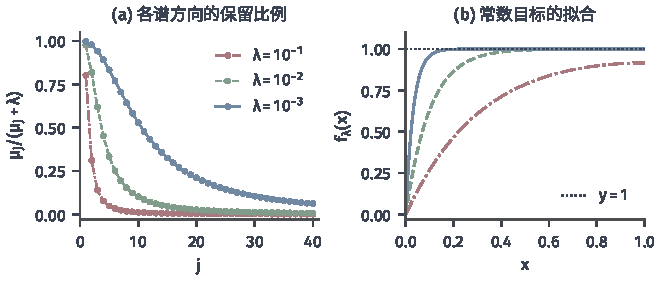
\includegraphics[width=112mm]{figures/03-optimization-evolution-and-signals/01-optimization/matplotlib/c8-spectral-shrinkage/figure.pdf}
  \caption{整体观测下的谱收缩，最小值核、$[0,1]$上Lebesgue测度，$\mu_j=((j-\tfrac12)\pi)^{-2}$。(a)~前$40$个谱方向的保留比例$\mu_j/(\mu_j+\lambda)$，$\lambda=10^{-1},10^{-2},10^{-3}$：比例随$j$平滑下降，没有在某个序号处截断。(b)~常数数据$y=1$（黑色点线）的拟合$f_\lambda$，线型与(a)对应；由于$H_{\min}$中的函数在$0$处为零，拟合在宽度约$\sqrt\lambda$的边界层内升起。三个$\lambda$下的有效维度$\sum_j\mu_j/(\mu_j+\lambda)$依次约为$1.58$、$5.00$、$15.81$。}
  \label{fig:opt-fit-spectral-shrinkage}
\end{figure}

\paragraph{正则化重新分配谱权重}
式~\eqref{eq:opt-fit-spectral-solution}说明，正则化对每个谱方向乘以因子$\mu_j/(\mu_j+\lambda)$。$\mu_j\gg\lambda$的方向几乎原样保留，$\mu_j\ll\lambda$的方向被压缩为原来的约$\mu_j/\lambda$。图~\ref{fig:opt-fit-spectral-shrinkage}(a)显示，因子随$j$平滑下降，并不在某个序号处由$1$突然变为$0$：正则化改变的是整个候选的频谱权重，而不是删去序号超过某个阈值的所有方向。这与第~\ref{sec:opt-fit-linear-basis}小节的岭回归滤波$\sigma_k^2/(\sigma_k^2+\lambda)$是同一种机制。有限个点值观测时也是如此：拟合读数$\bm G\bm a_\lambda=\bm G(\bm G+n\lambda\bm I)^{-1}\bm y$在$\bm G$的第$k$个特征方向上乘以$t_k/(t_k+n\lambda)$，$t_k$是Gram矩阵的特征值。有限Gram矩阵只有$n$个特征值，整体算子有无限多个；两者怎样随参数和数据变化，留到第~\ref{sec:opt-fit-error}节统一讨论。

\paragraph{有效维度}
把这些因子加起来，
\[
  N(\lambda)=\sum_j\frac{\mu_j}{\mu_j+\lambda},
\]
可以理解为在正则尺度$\lambda$下“有效保留”的谱方向个数：完全保留的方向计$1$，完全压掉的方向计$0$，部分保留的计其比例。称$N(\lambda)$为\term{有效维度}（effective dimension）。由于每项不超过$\mu_j/\lambda$，而Mercer定理保证$\sum_j\mu_j<\infty$（$T_K$是迹类算子），$N(\lambda)\le\lambda^{-1}\sum_j\mu_j<\infty$；即使谱方向有无限多个，有效维度也是有限数。对上面的最小值核，$\sum_j\mu_j=\tfrac12$，$\lambda=10^{-1},10^{-2},10^{-3}$时$N(\lambda)$约为$1.58$、$5.00$、$15.81$，大致按$1/(2\sqrt\lambda)$增长，远小于粗略上界$1/(2\lambda)$。

有效维度是给定核、测度与正则参数下的确定性量。它不是函数类的覆盖数，也不是实际计算时使用的特征个数；整体观测下的这个确定性结论，也不能自动变成有限随机样本下的泛化保证。

\subsection{导数观测下的拟合}
\label{sec:opt-fit-gradient-observations}

\paragraph{问题}
设$\Omega\subset\mathbb R^d$是有界连通的Lipschitz区域，给定向量场$\bm v\in L^2(\Omega;\mathbb R^d)$，以及一个$g\in H^1(\Omega)$，用它的边界迹规定边界值。要在边界值固定的函数中找梯度最接近$\bm v$的一个：
\begin{equation}
  \min_{u\in g+H_0^1(\Omega)}\ \frac12\|\nabla u-\bm v\|_{L^2(\Omega)}^2 .
  \label{eq:opt-fit-gradient-problem}
\end{equation}
这里用到的弱导数、Sobolev空间$H^1$与$H_0^1$、边界迹以及Poincaré不等式，可参考\BookChapterRef{chap:weak-derivatives-sobolev}{卷二“弱导数与Sobolev空间”章}。需要的结论是：存在常数$C_\Omega$，使所有$w\in H_0^1(\Omega)$满足$\|w\|_{L^2}\le C_\Omega\|\nabla w\|_{L^2}$。

\paragraph{化为投影}
令$u=g+w$，$w\in H_0^1(\Omega)$，目标变成$\tfrac12\|\nabla w-(\bm v-\nabla g)\|_{L^2}^2$。记
\[
  V=\{\nabla w:w\in H_0^1(\Omega)\}\subseteq L^2(\Omega;\mathbb R^d),
\]
问题就是求$\bm v-\nabla g$到$V$的最近点。$V$是线性子空间；要用投影定理，还需要它是闭的。

\begin{lemma}[梯度像是闭子空间]
\label{lem:opt-fit-gradient-closed}
$V$在$L^2(\Omega;\mathbb R^d)$中闭，且映射$w\mapsto\nabla w$在$H_0^1(\Omega)$上单射。
\end{lemma}

\begin{proof}
设$w_k\in H_0^1$，$\nabla w_k\to\bm z$于$L^2$。则$(\nabla w_k)$是Cauchy列。由Poincaré不等式，$\|w_k-w_m\|_{L^2}\le C_\Omega\|\nabla w_k-\nabla w_m\|_{L^2}$，所以$\|w_k-w_m\|_{H^1}^2=\|w_k-w_m\|_{L^2}^2+\|\nabla(w_k-w_m)\|_{L^2}^2\le(1+C_\Omega^2)\|\nabla w_k-\nabla w_m\|_{L^2}^2$，$(w_k)$是$H^1$中的Cauchy列。$H^1$完备，$H_0^1$是它的闭子空间，于是$w_k\to w\in H_0^1$于$H^1$，特别地$\nabla w_k\to\nabla w$于$L^2$。由极限唯一，$\bm z=\nabla w\in V$。单射性：若$\nabla w=\bm 0$，Poincaré不等式给出$\|w\|_{L^2}=0$。
\end{proof}

\begin{theorem}[梯度场拟合]
\label{thm:opt-fit-gradient}
问题~\eqref{eq:opt-fit-gradient-problem}有唯一解$u^\star=g+w^\star$，其中$\nabla w^\star$是$\bm v-\nabla g$在$V$上的正交投影。解由正交条件刻画：
\begin{equation}
  \int_\Omega(\nabla u^\star-\bm v)\cdot\nabla h\,\mathrm dx=0\qquad\text{对一切}\ h\in H_0^1(\Omega).
  \label{eq:opt-fit-gradient-orthogonality}
\end{equation}
\end{theorem}

\begin{proof}
由引理~\ref{lem:opt-fit-gradient-closed}，$V$是Hilbert空间$L^2(\Omega;\mathbb R^d)$的闭子空间，投影定理给出唯一的最近点$\bm z^\star\in V$，它由$\bm v-\nabla g-\bm z^\star\perp V$刻画。再由单射性，$\bm z^\star=\nabla w^\star$中的$w^\star\in H_0^1$唯一。$u\in g+H_0^1$与$w=u-g$一一对应，目标值相同，所以$u^\star=g+w^\star$是唯一解。正交条件$\langle\bm v-\nabla g-\nabla w^\star,\nabla h\rangle_{L^2}=0$对一切$h\in H_0^1$成立，即式~\eqref{eq:opt-fit-gradient-orthogonality}。
\end{proof}

推导中没有对$u$求任何泛函导数，也不要求$\bm v$恰好是某个函数的梯度；数据场中不是梯度的部分，就留在与$V$正交的余项里。

\paragraph{一维与二维的例子}
在$\Omega=(0,1)$上取$g=0$，即要求$u(0)=u(1)=0$。此时$V=\{w':w\in H_0^1(0,1)\}$恰是均值为零的$L^2$函数：$w(1)-w(0)=\int_0^1w'=0$；反过来，任一零均值的$z\in L^2$的原函数$\int_0^xz$属于$H_0^1$。到零均值子空间的投影就是减去均值，所以$(u^\star)'=v-\int_0^1v$。例如$v\equiv1$时$u^\star=0$，余项$v-(u^\star)'=1$与每个$h'$（$h\in H_0^1$）正交，因为$\int_0^1h'=0$：固定的边界值不允许函数整体爬升，常数斜率完全无法被吸收。

二维时，余项可以是“旋转”的。在单位正方形上取$\varphi=\sin\pi x\sin\pi y$（它属于$H_0^1$）与$\psi=0.8\varphi$，令
\[
  \bm v=\nabla\varphi+(\partial_y\psi,\,-\partial_x\psi).
\]
对$h\in C_c^\infty$，分部积分得$\int(\partial_y\psi\,\partial_xh-\partial_x\psi\,\partial_yh)=-\int(\partial_x\partial_y\psi-\partial_y\partial_x\psi)h=0$，再由稠密性推广到一切$h\in H_0^1$。所以第二项与$V$正交，而$\nabla\varphi\in V$，投影恰好是$\nabla\varphi$，$u^\star=\varphi$。图~\ref{fig:opt-fit-gradient-projection}把三个场并排画出：给定场同时有发散与旋转，投影保留了从中心向外的“梯度部分”，余项则是绕中心旋转的场，它不是任何函数的梯度，拟合无法也不应吸收它。

\begin{figure}[!htbp]
  \centering
  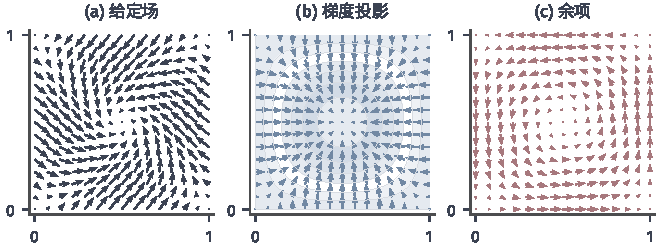
\includegraphics[width=112mm]{figures/03-optimization-evolution-and-signals/01-optimization/matplotlib/c8-gradient-projection/figure.pdf}
  \caption{单位正方形上的梯度场拟合，零边界值。(a)~给定场$\bm v=\nabla\varphi+(\partial_y\psi,-\partial_x\psi)$，$\varphi=\sin\pi x\sin\pi y$，$\psi=0.8\sin\pi x\sin\pi y$；(b)~它在$V=\{\nabla w:w\in H_0^1\}$上的投影$\nabla u^\star=\nabla\varphi$，底色为$u^\star=\varphi$的等值区域；(c)~余项$\bm v-\nabla u^\star=(\partial_y\psi,-\partial_x\psi)$，它与$V$正交，是绕中心旋转的场。箭头长度按同一比例缩放。}
  \label{fig:opt-fit-gradient-projection}
\end{figure}

\paragraph{自由边界}
若不规定边界值，在整个$H^1(\Omega)$中极小化$\tfrac12\|\nabla u-\bm v\|^2$，加任意常数不改变目标，解至多唯一到常数。改在零均值子空间$\{u\in H^1:\int_\Omega u=0\}$中求解，用Poincaré--Wirtinger不等式$\|u-u_\Omega\|_{L^2}\le C\|\nabla u\|_{L^2}$（$u_\Omega$为均值，这里需要$\Omega$连通）代替上面的Poincaré不等式，同样的论证说明梯度像闭、映射单射，于是存在唯一的零均值解，一般解为它加任意常数。在$(0,1)$上，任何$v\in L^2$都是其原函数的导数，于是自由边界的解满足$u'=v$，余项为零，与固定边界的情形形成对照。把正交条件~\eqref{eq:opt-fit-gradient-orthogonality}改写成区域内的方程与边界条件（自由边界时出现自然边界条件），需要分部积分和泛函微分的语言，留给第~\ref{chap:opt-functional}章；那里不再重复建立这个问题的求解理论。

\section{拟合误差与稳定性}
\label{sec:opt-fit-error}

前面每个定理给出的都是某个精确问题的精确解。实际得到的函数还受三类因素影响：读数本身有扰动，正则参数需要选择，计算只能在有限的表示中、用有限的迭代完成。这三者改变的对象不同，度量它们的范数也不同。本节固定同一个观测任务，把它们一一分开：先在固定的$\lambda$下看数据扰动怎样传到最优函数，再看$\lambda$本身怎样决定拟合程度，最后区分表示受限与计算未完成两种误差。

\subsection{固定正则参数下的数据扰动}
\label{sec:opt-fit-data-perturbation}

\paragraph{有限观测}
固定有界观测$L$、Gram矩阵$\bm G$与$\lambda>0$，比较数据$\bm y$与$\bm y+\delta\bm y$下的两个精确解。由定理~\ref{thm:opt-fit-kernel-ridge}，规范系数之差为$\delta\bm a=(\bm G+n\lambda\bm I)^{-1}\delta\bm y$，函数之差$\delta f=\sum_j\delta a_jh_j$。

\begin{theorem}[有限观测下的数据稳定性]
\label{thm:opt-fit-data-stability}
在上述设定下，
\[
  \|\delta f\|_H\le\frac{\|\delta\bm y\|_2}{2\sqrt{n\lambda}},\qquad
  \|L\,\delta f\|_2\le\|\delta\bm y\|_2 .
\]
\end{theorem}

\begin{proof}
设$\bm G=\sum_kt_k\bm u_k\bm u_k^\top$是谱分解，$t_k\ge0$，$\{\bm u_k\}$标准正交。由式~\eqref{eq:opt-fit-gram-calculus}，
\[
  \|\delta f\|_H^2=\delta\bm a^\top\bm G\,\delta\bm a=\sum_k\frac{t_k}{(t_k+n\lambda)^2}(\bm u_k^\top\delta\bm y)^2 .
\]
函数$t\mapsto t/(t+c)^2$在$t\ge0$上的最大值是$1/(4c)$，在$t=c$处取到（求导可得），取$c=n\lambda$即得第一式。读数之差$L\delta f=\bm G\delta\bm a=\sum_kt_k(t_k+n\lambda)^{-1}(\bm u_k^\top\delta\bm y)\bm u_k$，每个因子不超过$1$，得第二式。
\end{proof}

谱权重$t/(t+n\lambda)^2$解释了这个界从哪里来。很大的特征方向被数据项牢牢约束，扰动在那里被$1/t$压小；很小的特征方向被正则项压住；最危险的是$t\approx n\lambda$的中间方向，两种力量都不强。$\lambda$越小，这个最坏的放大倍数$1/(2\sqrt{n\lambda})$越大。

在例~\ref{ex:opt-fit-min-kernel}中取$\delta\bm y=(\varepsilon,0)^\top$，$n\lambda=\tfrac12$。$\delta\bm a=(\bm G+\tfrac12\bm I)^{-1}\delta\bm y=(\tfrac65,-\tfrac25)^\top\varepsilon$，$\bm G\delta\bm a=(\tfrac25,\tfrac15)^\top\varepsilon$，于是$\|\delta f\|_H^2=\delta\bm a^\top\bm G\delta\bm a=(\tfrac{12}{25}-\tfrac2{25})\varepsilon^2=0.4\varepsilon^2$，$\|\delta f\|_H\approx0.632\varepsilon$，在界$\varepsilon/\sqrt2\approx0.707\varepsilon$之内。图~\ref{fig:opt-fit-data-perturbation}在一个十二点的高斯核例子上比较两个$\lambda$：只把一个读数上移$0.4$，$\lambda=10^{-7}$时函数在扰动点两侧都出现起伏，$\|\delta f\|_H\approx16.3$；$\lambda=10^{-2}$时变化平缓而局部，$\|\delta f\|_H\approx0.33$。

\begin{figure}[!htbp]
  \centering
  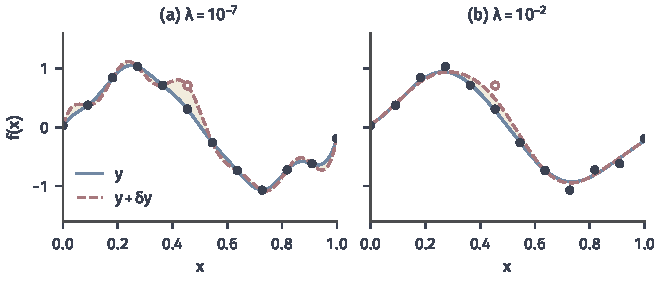
\includegraphics[width=112mm]{figures/03-optimization-evolution-and-signals/01-optimization/matplotlib/c8-data-perturbation/figure.pdf}
  \caption{固定$\lambda$下数据扰动对拟合的影响。高斯核（$\sigma=0.15$），$x_i=i/11$（$i=0,\dots,11$），教学示例读数$y_i=\sin2\pi x_i$加固定种子的$N(0,0.1^2)$噪声（黑点）；只把第六个读数上移$0.4$（空心点）。蓝线与红色虚线分别为扰动前后的核岭回归解，黄色区域为两者之差。(a)~$\lambda=10^{-7}$：$\|\delta f\|_H\approx16.3$，界$\|\delta\bm y\|_2/(2\sqrt{n\lambda})\approx183$；(b)~$\lambda=10^{-2}$：$\|\delta f\|_H\approx0.33$，界约为$0.58$。}
  \label{fig:opt-fit-data-perturbation}
\end{figure}

\paragraph{整体观测}
对第~\ref{sec:opt-fit-function-values}小节的整体观测，数据扰动$\delta y$的谱坐标$\delta c_j$经过同一个乘子：$\delta b_j=\mu_j\delta c_j/(\mu_j+\lambda)$。由此
\[
  \begin{gathered}
  \|\delta f\|_{L^2}^2=\sum_j\Bigl(\frac{\mu_j}{\mu_j+\lambda}\Bigr)^2\delta c_j^2\le\|\delta y\|_{L^2}^2,\\
  \|\delta f\|_H^2=\sum_j\frac{\mu_j}{(\mu_j+\lambda)^2}\delta c_j^2\le\frac{\|\delta y\|_{L^2}^2}{4\lambda}.
  \end{gathered}
\]
同一个扰动在两个范数下有不同的稳定常数：$L^2$中不放大，$H$中最多放大$1/(2\sqrt\lambda)$倍。原因是$H$范数给小特征值方向更重的权重$1/\mu_j$，而这些方向恰是$\lambda$小时最容易被数据带动的方向。

\paragraph{这些界比较的是什么}
两个界比较的是两个精确问题的精确解，对象、核、观测位置与$\lambda$都固定。若改变观测位置、测度或核，$\bm G$、算子乃至表示元本身都变了，需要另外控制这些对象的扰动，不能继续套用上面只针对数据的公式。求解器的舍入误差也是另一回事：它取决于线性系统$\bm G+n\lambda\bm I$的条件数，后者不超过$(t_{\max}+n\lambda)/(n\lambda)$；原问题对数据的敏感性和算法的数值稳定性应分别评价。

\subsection{正则参数与拟合程度}
\label{sec:opt-fit-lambda}

\paragraph{$\lambda\downarrow0$的极限：有限观测}
固定数据，让正则参数趋于零。在$\bm G$的特征坐标中，规范系数为$\bm a_\lambda=\sum_k(t_k+n\lambda)^{-1}(\bm u_k^\top\bm y)\bm u_k$。零特征值方向上的分量是$(n\lambda)^{-1}\bm u_k^\top\bm y$，它会发散，但由于$\ker\bm G$中的系数不改变函数，它对$f_\lambda$没有贡献。只看正特征值，令$f^\dagger=\sum_j(\bm G^\dagger\bm y)_jh_j$，
\[
  \|f_\lambda-f^\dagger\|_H^2=\sum_{t_k>0}t_k\Bigl(\frac1{t_k+n\lambda}-\frac1{t_k}\Bigr)^2(\bm u_k^\top\bm y)^2\longrightarrow0 .
\]
所以$f_\lambda\to f^\dagger$于$H$。$f^\dagger$是在所有使$\|Lf-\bm y\|_2$最小的函数中范数最小的一个：读数$\bm G\bm a$能达到的最近点是$\bm y$在$\operatorname{range}\bm G$上的投影$\bm G\bm G^\dagger\bm y$，而在读数等于它的函数中，按定理~\ref{thm:opt-fit-min-norm-interpolation}的论证，$f^\dagger$范数最小。若$\bm y\in\operatorname{range}\bm G$，$f^\dagger$就是最小范数插值，这正是图~\ref{fig:opt-fit-min-kernel}(a)中红色虚线的来历；若$\bm y\notin\operatorname{range}\bm G$，极限的残差是$\|(\bm I-\bm G\bm G^\dagger)\bm y\|_2>0$，不应称为插值。

\paragraph{$\lambda\downarrow0$的极限：整体观测}
整体观测下，$b_j^\star=\mu_jc_j/(\mu_j+\lambda)\to c_j$。在$L^2$中，$\|f_\lambda-\sum_jc_j\psi_j\|_{L^2}^2=\sum_j\bigl(\lambda c_j/(\mu_j+\lambda)\bigr)^2$，每项不超过$c_j^2$且逐项趋于零，由控制收敛（对级数），极限为零：$f_\lambda$在$L^2$中收敛到$y$在可表示方向的闭包上的投影$y-y_0$。在$H$中则不然：$\|f_\lambda\|_H^2=\sum_j\mu_jc_j^2/(\mu_j+\lambda)^2$随$\lambda\downarrow0$单调增加到$\sum_jc_j^2/\mu_j$。只有当这个和有限，即$y-y_0\in H$时，$f_\lambda$才在$H$中收敛；否则$H$范数趋于无穷。在最小值核的例子中$y=1$，$\sum_jc_j^2/\mu_j=\sum_j2=\infty$：拟合在$L^2$中趋于$1$，在$H_{\min}$中却越来越“贵”，与图~\ref{fig:opt-fit-spectral-shrinkage}(b)中越来越陡的边界层相符。这里讨论的是精确解随参数变化的极限，它和迭代算法的轨迹极限是两回事，后者在第~\ref{sec:opt-fit-implicit-bias}节讨论。

\paragraph{残差与范数的此消彼长}
固定数据，比较不同$\lambda$下的读数残差与函数范数。在$\bm G$的特征坐标中，
\[
  \bm G\bm a_\lambda-\bm y=-\sum_k\frac{n\lambda}{t_k+n\lambda}(\bm u_k^\top\bm y)\bm u_k,\qquad
  \|f_\lambda\|_H^2=\sum_k\frac{t_k}{(t_k+n\lambda)^2}(\bm u_k^\top\bm y)^2 .
\]
第一式每个系数随$\lambda$增大，第二式每项随$\lambda$减小，所以残差范数$\|Lf_\lambda-\bm y\|_2$关于$\lambda$单调不减，函数范数$\|f_\lambda\|_H$单调不增。把每个$\lambda$对应的一对数画在双对数坐标中，得到的曲线常呈“L”形，称为\term{L曲线}（L-curve）。图~\ref{fig:opt-fit-lcurve}在十五个带噪读数上画出了解族与L曲线：$\lambda=10^{-7}$时残差只有$0.07$，函数范数却达到$41$，曲线贴着每个点抖动；$\lambda=10^{-1}$时范数降到约$0.95$，残差升到$0.92$，曲线被明显压平。

\paragraph{残差匹配原则}
若事先知道读数误差的确定性上界$\|\bm e\|_2\le\delta$，一个自然的选择是不要求残差比误差更小：取$\lambda$使$\|Lf_\lambda-\bm y\|_2=\delta$。由上面的单调性和连续性，当$\|(\bm I-\bm G\bm G^\dagger)\bm y\|_2<\delta<\|\bm y\|_2$时，这样的$\lambda$存在。这一做法称为\term{残差匹配原则}（discrepancy principle）。图~\ref{fig:opt-fit-lcurve}中的教学数据是人为加噪的，误差向量已知，$\|\bm e\|_2\approx0.559$，按此原则得到$\lambda\approx2.8\times10^{-2}$（绿色），它在L曲线上位于拐角附近。实际问题中通常只有误差的估计，这时原则的结论依赖于估计是否可靠。

\begin{figure}[!htbp]
  \centering
  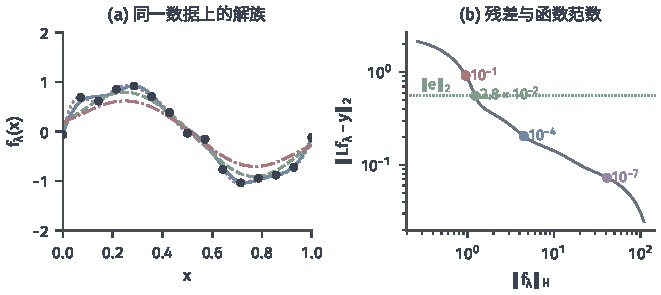
\includegraphics[width=112mm]{figures/03-optimization-evolution-and-signals/01-optimization/matplotlib/c8-lcurve/figure.pdf}
  \caption{正则参数决定拟合程度。高斯核（$\sigma=0.15$），教学示例数据为$x_i=i/14$上的$\sin2\pi x_i$加固定种子的$N(0,0.15^2)$噪声，$n=15$。(a)~$\lambda=10^{-7}$（紫色点线）、$10^{-4}$（蓝线）、$2.8\times10^{-2}$（绿色虚线）、$10^{-1}$（红色点划线）的核岭回归解。(b)~L曲线：横轴为函数范数$\|f_\lambda\|_H$，纵轴为读数残差$\|Lf_\lambda-\bm y\|_2$，均为对数刻度；圆点对应(a)中的四个$\lambda$，绿色点线为噪声范数$\|\bm e\|_2\approx0.559$，残差与之相等处即残差匹配原则选出的$\lambda$。}
  \label{fig:opt-fit-lcurve}
\end{figure}

\paragraph{这里不讨论预测保证}
无论L曲线还是残差匹配原则，都只用到训练读数和确定性的误差界。基于随机样本的交叉验证、使期望风险最小的参数以及统计一致性，需要关于数据生成机制的假设，属于统计学习理论的问题，可参考\BookChapterRef{chap:statistical-learning-framework}{卷六“机器学习理论基础”章}。不能由训练残差小推出预测误差小。

\subsection{表示误差与计算误差}
\label{sec:opt-fit-representation-computation}

\paragraph{两种差值}
固定候选空间$H$与目标$J$，记精确最优值$J^\star=\inf_HJ$。算法返回某个$\hat f$，差值$J(\hat f)-J^\star$称为优化误差，它来自算法没有解完。另一方面，若为了计算把候选限制到子空间$H_m\subseteq H$（例如$m$个特征张成的空间），即使在$H_m$中精确求解，所得最优值$J_m^\star=\inf_{H_m}J$也可能大于$J^\star$，差值$J_m^\star-J^\star\ge0$称为表示误差，它来自候选集合受限。在$H_m$中计算得到$\hat f_m$时，
\[
  J(\hat f_m)-J^\star=\underbrace{\bigl(J(\hat f_m)-J_m^\star\bigr)}_{\text{优化误差}}+\underbrace{\bigl(J_m^\star-J^\star\bigr)}_{\text{表示误差}},
\]
两项都以同一个目标值度量，所以可以相加。若关心的是函数之间的距离，就需要一个把目标值差转成距离的条件，不能把一个目标值差和一个范数距离直接相加。

\paragraph{目标值差控制函数距离}
对平方拟合目标~\eqref{eq:opt-fit-kernel-ridge}，这个条件可以精确写出。对任意$f\in H$，令$g=f-f_\lambda$，展开得
\[
  J(f_\lambda+g)=J(f_\lambda)+2\Bigl[\frac1n\langle Lf_\lambda-\bm y,Lg\rangle+\lambda\langle f_\lambda,g\rangle_H\Bigr]+\frac1n\|Lg\|_2^2+\lambda\|g\|_H^2 .
\]
方括号为零：由$L_ig=\langle g,h_i\rangle$与$f_\lambda=\sum_ja_jh_j$，它等于$\bigl\langle\sum_j[\tfrac1n(\bm G\bm a-\bm y)_j+\lambda a_j]h_j,\,g\bigr\rangle_H$，而规范系数满足$(\bm G+n\lambda\bm I)\bm a=\bm y$，括号内每个系数都是零。于是
\begin{equation}
  J(f)-J(f_\lambda)=\frac1n\|L(f-f_\lambda)\|_2^2+\lambda\|f-f_\lambda\|_H^2\ \ge\ \lambda\|f-f_\lambda\|_H^2 .
  \label{eq:opt-fit-objective-gap}
\end{equation}
任何近似解的目标值差都直接给出它到精确解的$H$距离上界，表示误差和优化误差可以先在目标值中相加，再通过这个不等式换成距离。

\paragraph{有限特征与提前停止改变不同的对象}
观测数很大时有两类常见的省算办法。一类是有限特征近似：用$m\ll n$个特征张成$H_m$，或用低秩矩阵代替$\bm G$；前者限制了候选集合，后者改变了目标本身，误差应相对于各自声明的精确问题评价。另一类是\term{提前终止}（early stopping）：在完整的$n$维系数问题上运行梯度法或CG，迭代若干轮后停下；候选集合与目标都没变，留下的是优化误差。两者都减少了计算量，但前者的误差不会随迭代增加而消失，后者的误差会；把它们都称为“近似”而不说明改变了什么，就无法判断结果相对于哪个问题可信。

\paragraph{系数误差与函数误差}
在固定的Gram矩阵下迭代求系数时，系数误差与函数误差由式~\eqref{eq:opt-fit-gram-calculus}联系：
\[
  \begin{gathered}
  \|f_{\bm a}-f_{\bm b}\|_H^2=(\bm a-\bm b)^\top\bm G(\bm a-\bm b)\le\|\bm G\|_2\,\|\bm a-\bm b\|_2^2,\\
  |L_i(f_{\bm a}-f_{\bm b})|\le\|h_i\|_H\,\|f_{\bm a}-f_{\bm b}\|_H=\sqrt{\bm G_{i,i}}\,\|f_{\bm a}-f_{\bm b}\|_H .
  \end{gathered}
\]
所以系数收敛推出函数收敛，函数收敛又推出每个读数收敛。反过来不成立：$\bm G$奇异时，系数可以沿$\ker\bm G$漂移而函数不变，例如仿射核例子中$\bm a+c(1,-2,1)^\top$对任何$c$都给出同一函数。因此停止准则应按关心的量来定：关心读数时监控$\bm G\bm a$，关心函数时监控Gram二次型，不必要求系数本身收敛。

对线性系统$(\bm G+n\lambda\bm I)\bm a=\bm y$的近似解$\bm a$，记残差$\bm s=(\bm G+n\lambda\bm I)\bm a-\bm y$。则$\bm a-\bm a_\lambda=(\bm G+n\lambda\bm I)^{-1}\bm s$，与数据扰动$\delta\bm y=\bm s$时的系数差完全相同，由定理~\ref{thm:opt-fit-data-stability}，
\[
  \|f_{\bm a}-f_\lambda\|_H\le\frac{\|\bm s\|_2}{2\sqrt{n\lambda}} .
\]
未解完的计算误差，在函数层面表现得就像一次大小为$\|\bm s\|_2$的数据扰动。在例~\ref{ex:opt-fit-min-kernel}中，若迭代停在线性残差$\bm s=(\varepsilon,0)^\top$处，上一小节的计算说明函数误差约为$0.632\varepsilon$。于是，若希望计算误差不超过数据本身的不确定性，可以要求$\|\bm s\|_2$不超过已知的读数误差量级，而不必追求机器精度。

\section{迭代选解与隐式偏置}
\label{sec:opt-fit-implicit-bias}

第一节说过，读数看不见的方向要由额外的偏好来确定。前面的偏好都写在目标里。可是在过参数化的拟合中，人们常常不加任何正则，直接用梯度法极小化数据误差；此时目标有无穷多个最小点，或者根本没有有限的最小点，算法还是会交出一个确定的结果。本节研究这个结果由什么决定。由优化过程本身产生、没有写进目标的选择偏好，称为\term{隐式偏差}（implicit bias），也常称隐式偏置。我们先在最小二乘中完整证明它，再以补充的形式说明分类和矩阵因子化中的相应现象及其适用边界。

\subsection{最小二乘中的初值与尺度}
\label{sec:opt-fit-implicit-least-squares}

\paragraph{梯度永远在行空间中}
考虑$F(\bm w)=\frac1{2n}\|\bm X\bm w-\bm y\|_2^2$，$\bm X\in\mathbb R^{n\times d}$可以有$d>n$。它的梯度$\nabla F(\bm w)=\bm X^\top(\bm X\bm w-\bm y)/n$总属于$\operatorname{range}(\bm X^\top)=(\ker\bm X)^\perp$。梯度下降$\bm w^{(t+1)}=\bm w^{(t)}-\eta\nabla F(\bm w^{(t)})$每步只沿行空间移动，所以$\bm w^{(t)}$在$\ker\bm X$上的投影始终等于初值的投影：数据看不见的方向，算法也从不触碰。

\begin{theorem}[梯度下降的最小二乘极限]
\label{thm:opt-fit-gd-limit}
设$\bm X\ne\bm 0$，步长$0<\eta<2n/\|\bm X\|_2^2$。则对任意初值$\bm w^{(0)}$，
\[
  \bm w^{(t)}\to\bm X^\dagger\bm y+P_{\ker\bm X}\bm w^{(0)} .
\]
特别地，零初值时极限是$\bm X^\dagger\bm y$，即所有最小二乘解中欧氏范数最小的一个。
\end{theorem}

\begin{proof}
设$\bm X=\sum_{k=1}^r\sigma_k\bm u_k\bm v_k^\top$，$\sigma_1\ge\cdots\ge\sigma_r>0$，把$\{\bm v_1,\dots,\bm v_r\}$补成$\mathbb R^d$的标准正交基。记坐标$z_k=\bm v_k^\top\bm w$。对$k\le r$，$\bm v_k^\top\bm X^\top(\bm X\bm w-\bm y)=\sigma_k(\sigma_kz_k-\bm u_k^\top\bm y)$，令$z_k^\star=\bm u_k^\top\bm y/\sigma_k$，更新化为
\[
  z_k^{(t+1)}-z_k^\star=\Bigl(1-\frac{\eta\sigma_k^2}n\Bigr)\bigl(z_k^{(t)}-z_k^\star\bigr).
\]
由$0<\eta\sigma_k^2/n\le\eta\sigma_1^2/n<2$，因子的绝对值小于$1$，$z_k^{(t)}\to z_k^\star$。对$k>r$，$\bm v_k\in\ker\bm X$，梯度在该坐标上为零，$z_k^{(t)}=z_k^{(0)}$。合起来，极限为$\sum_{k\le r}z_k^\star\bm v_k+\sum_{k>r}z_k^{(0)}\bm v_k=\bm X^\dagger\bm y+P_{\ker\bm X}\bm w^{(0)}$。$\bm X^\dagger\bm y$是最小范数最小二乘解，见前文引用的卷一“线性方程与矩阵方程”章。
\end{proof}

定理没有假设数据可以被精确插值：$\bm y\notin\operatorname{range}\bm X$时，极限仍是最小二乘解，只是残差不为零。非零初值时，算法选出的是离初值最近的最小二乘解。

\paragraph{预条件改变被选中的解}
把更新改为$\bm w^{(t+1)}=\bm w^{(t)}-\eta\bm P\nabla F(\bm w^{(t)})$，$\bm P$是固定的对称正定矩阵。令$\bm w=\bm P^{1/2}\bm z$，更新变为
\[
  \bm z^{(t+1)}=\bm z^{(t)}-\frac\eta n\bm P^{1/2}\bm X^\top\bigl(\bm X\bm P^{1/2}\bm z^{(t)}-\bm y\bigr),
\]
它是对$\frac1{2n}\|\tilde{\bm X}\bm z-\bm y\|_2^2$（$\tilde{\bm X}=\bm X\bm P^{1/2}$）的普通梯度下降。由定理~\ref{thm:opt-fit-gd-limit}，在$0<\eta<2n/\|\bm X\bm P^{1/2}\|_2^2$时，零初值的$\bm z^{(t)}$收敛到使$\|\bm z\|_2$最小的最小二乘解。$\bm z\mapsto\bm P^{1/2}\bm z$把两组最小二乘解一一对应，且$\|\bm z\|_2^2=\bm w^\top\bm P^{-1}\bm w$，所以$\bm w^{(t)}$收敛到使$\bm w^\top\bm P^{-1}\bm w$最小的最小二乘解。预条件不只改变速度，还改变了被选中的解。

\begin{example}[同一条直线上的两个选择]
\label{ex:opt-fit-implicit-preconditioner}
取$n=1$，$\bm X=(1,1)$，$y=1$，最小二乘解（此处即插值解）是直线$w_1+w_2=1$上的全部点，目标值都为零。$\bm P=\bm I$时，步长条件为$\eta<1$，零初值下的极限是最小欧氏范数解$(\tfrac12,\tfrac12)$。$\bm P=\operatorname{diag}(1,4)$时，步长条件为$\eta<2/5$，极限使$w_1^2+w_2^2/4$最小：由Lagrange条件$2w_1=\nu$、$w_2/2=\nu$得$w_2=4w_1$，再代入约束得$(\tfrac15,\tfrac45)$。
\end{example}

图~\ref{fig:opt-fit-implicit-bias-gd}画出了这两条轨迹。由于梯度总与$(1,1)$成比例，$\bm P=\bm I$的轨迹沿$(1,1)$方向直线前进，在与解直线相切的圆处停下；$\bm P=\operatorname{diag}(1,4)$的轨迹沿$\bm P(1,1)^\top=(1,4)^\top$方向前进，停在与解直线相切的椭圆$w_1^2+w_2^2/4=\tfrac15$上。从$(1.2,-0.5)$出发的绿色轨迹则沿$(1,1)$方向落到$(1.35,-0.35)$，它保留了初值在$\ker\bm X=\operatorname{span}\{(1,-1)^\top\}$上的分量。

\begin{figure}[!htbp]
  \centering
  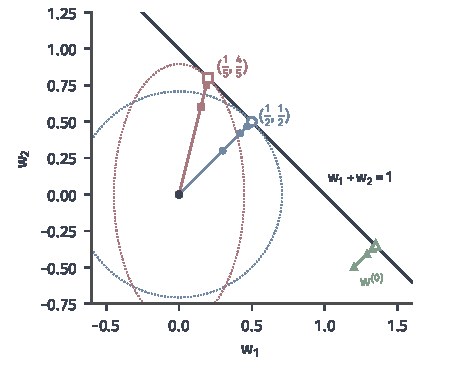
\includegraphics[width=80mm]{figures/03-optimization-evolution-and-signals/01-optimization/matplotlib/c8-implicit-bias-gd/figure.pdf}
  \caption{欠定最小二乘$\tfrac12(w_1+w_2-1)^2$上梯度下降的极限。黑线为全部最小点$w_1+w_2=1$。蓝色轨迹：$\bm P=\bm I$、$\eta=0.3$、零初值，收敛到$(\tfrac12,\tfrac12)$，蓝色点线圆$\|\bm w\|_2^2=\tfrac12$与黑线相切于此；红色轨迹：$\bm P=\operatorname{diag}(1,4)$、$\eta=0.15$、零初值，收敛到$(\tfrac15,\tfrac45)$，红色点线椭圆$w_1^2+w_2^2/4=\tfrac15$与黑线相切于此；绿色轨迹：$\bm P=\bm I$、初值$(1.2,-0.5)$，收敛到$(1.35,-0.35)$。标记为前几次迭代，空心标记为极限。}
  \label{fig:opt-fit-implicit-bias-gd}
\end{figure}

\paragraph{隐式选择不等于显式正则化}
零初值梯度下降的极限$\bm X^\dagger\bm y$恰好是岭回归解在$\lambda\downarrow0$时的极限，但这并不意味着两者在其他参数下也一致。仍以$\bm X=(1,1)$、$y=1$为例，$\lambda=1$的岭回归解是$(\bm X^\top\bm X+\bm I)^{-1}\bm X^\top y=(\tfrac13,\tfrac13)$，它根本不是最小二乘解；梯度下降在任何有限步停下的点也与任何一个$\lambda$的岭回归解一般不重合，除非像本例这样整条轨迹恰好落在同一条射线上。隐式偏好描述的是“算法在最小点集合中选哪一个”，显式正则化则改变了最小点集合本身。

\subsection{可分分类中的方向选择（补充）}
\label{sec:opt-fit-separable}

\paragraph{没有有限的最小点}
在二分类中，数据$(\bm x_i,y_i)$，$y_i\in\{-1,1\}$，用齐次线性预测器$\bm w^\top\bm x$与logistic损失，目标为
\[
  F(\bm w)=\frac1n\sum_{i=1}^n\log\bigl(1+\exp(-y_i\bm w^\top\bm x_i)\bigr).
\]
设数据严格线性可分，即存在$\bar{\bm w}$使$y_i\bar{\bm w}^\top\bm x_i>0$对所有$i$成立。沿这个方向放大参数，$F(s\bar{\bm w})\to0$（$s\to\infty$）；而每一项都严格为正，任何有限的$\bm w$都有$F(\bm w)>0$。所以下确界$0$达不到，问题没有有限的最小点，梯度下降的参数范数必然趋于无穷。这时有意义的问题不再是“参数收敛到哪个最小点”，而是“参数的方向趋于哪里”。

\paragraph{方向趋于硬间隔解}
Soudry等人证明\scite{soudry2018implicit}：在上述设定下，对欧氏全批量梯度下降，取充分小的固定步长（例如小于$2/\beta$，$\beta$为$F$梯度的Lipschitz常数，对logistic损失可取$\|\bm X\|_2^2/(4n)$，$\bm X$的行是$\bm x_i^\top$），从任意初值出发，都有$\|\bm w^{(t)}\|_2\to\infty$且
\[
  \frac{\bm w^{(t)}}{\|\bm w^{(t)}\|_2}\to\frac{\hat{\bm w}}{\|\hat{\bm w}\|_2},\qquad
  \hat{\bm w}=\argmin_{\bm w}\Bigl\{\|\bm w\|_2^2:\ y_i\bm w^\top\bm x_i\ge1,\ i=1,\dots,n\Bigr\}.
\]
$\hat{\bm w}$是\term{硬间隔}（hard margin）支持向量机的解：在所有把每个样本的间隔推到至少$1$的方向中，它的范数最小，也就是几何间隔最大。方向收敛只以对数速率进行，非常缓慢。

图~\ref{fig:opt-fit-separable}给出一个六点的例子。硬间隔解为$\hat{\bm w}=(0.8,0.4)$，唯一的支持向量是$(-1,-0.5)$。从零初值、步长$\eta=1$出发（这里$\|\bm X\|_2^2/(4n)\approx1.66$，步长满足$\eta<2/\beta$），迭代方向与$\hat{\bm w}$的夹角在第$1$步约为$25^\circ$，第$1701$步约为$11.6^\circ$，到第$10^6$步仍有约$5.9^\circ$，此时$\|\bm w^{(t)}\|_2\approx11.0$。迭代次数每增加数十倍，夹角才减少几度。

\begin{figure}[!htbp]
  \centering
  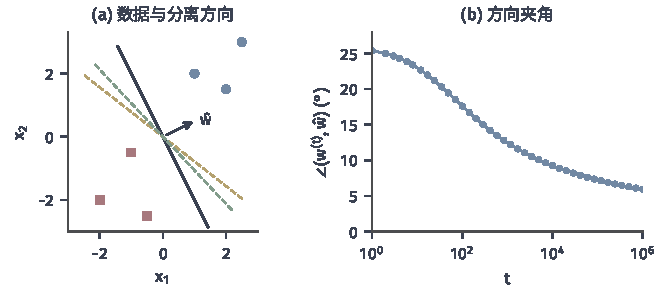
\includegraphics[width=112mm]{figures/03-optimization-evolution-and-signals/01-optimization/matplotlib/c8-separable-direction/figure.pdf}
  \caption{可分数据上logistic损失梯度下降的方向。(a)~正类（蓝色圆点）与负类（红色方块）各三个点；黑线为硬间隔解$\hat{\bm w}=(0.8,0.4)$对应的分界线，箭头为$\hat{\bm w}$的方向；黄色与绿色虚线为第$1$步与第$143$步迭代对应的分界线。(b)~迭代方向与$\hat{\bm w}$的夹角随迭代次数（对数刻度）的变化，零初值，$\eta=1$。}
  \label{fig:opt-fit-separable}
\end{figure}

\paragraph{结论的边界}
这个结论绑定于齐次线性预测器、指数型尾部的损失（logistic、指数损失）和欧氏梯度下降。换成尾部更重的损失、加入预条件或改用自适应方法，极限方向一般不同，需要重新分析。它只描述优化在无穷多个“近似最小点”中选择了什么，不直接给出测试误差；间隔与泛化的关系属于学习理论的内容。

\subsection{参数化、秩约束与谱选择的边界（补充）}
\label{sec:opt-fit-factorization}

\paragraph{因子化先规定了可表达的范围}
设要拟合的未知量是矩阵$\bm W\in\mathbb R^{p\times q}$。直接优化$\bm W$与写成$\bm W=\bm U\bm V^\top$（$\bm U\in\mathbb R^{p\times k}$，$\bm V\in\mathbb R^{q\times k}$）再优化因子，是两个不同的问题。内部宽度$k$先规定了$\operatorname{rank}\bm W\le k$：这是显式的低秩候选集合，属于表达限制，不是算法的偏好。参数化还引入了冗余：$(c\bm U,\bm V/c)$对任何$c\ne0$都给出同一个$\bm W$，就像核系数沿$\ker\bm G$移动不改变函数一样。

\paragraph{因子上的惩罚是一种显式偏好}
在因子上加平方惩罚，等价于在$\bm W$上加核范数（奇异值之和）$\|\bm W\|_*$惩罚：当$k\ge\operatorname{rank}\bm W$时，
\[
  \|\bm W\|_*=\min_{\bm U\bm V^\top=\bm W}\ \frac12\bigl(\|\bm U\|_F^2+\|\bm V\|_F^2\bigr).
\]
证明如下。设$\bm W=\bm A\bm\Sigma\bm B^\top$是紧奇异值分解，$\bm A,\bm B$的列标准正交。对任何$\bm U\bm V^\top=\bm W$，$\|\bm W\|_*=\operatorname{tr}(\bm A^\top\bm W\bm B)=\langle\bm U^\top\bm A,\bm V^\top\bm B\rangle_F\le\|\bm U^\top\bm A\|_F\|\bm V^\top\bm B\|_F\le\|\bm U\|_F\|\bm V\|_F\le\tfrac12(\|\bm U\|_F^2+\|\bm V\|_F^2)$，其中第二个不等号用了$\bm A$、$\bm B$的列标准正交。取$\bm U=\bm A\bm\Sigma^{1/2}$、$\bm V=\bm B\bm\Sigma^{1/2}$（宽度不足$k$时补零列）各处取等。所以“因子化加权重衰减”是一个显式的核范数正则化问题，它与“不加惩罚、靠迭代形成的偏好”应当分开讨论。

\paragraph{因子化本身不保证低秩}
没有显式惩罚时，因子化的梯度法是否偏向低秩或小核范数，取决于初值、步长与问题结构，不能仅凭“用了因子化”下结论。一个例子：$F(\bm U,\bm V)=\tfrac12\|\bm U\bm V^\top-\bm I_2\|_F^2$，取$\bm U^{(0)}=\bm V^{(0)}=a^{(0)}\bm I_2$，$0<a^{(0)}<1$。对$\bm U$的梯度是$(\bm U\bm V^\top-\bm I)\bm V=(a^2-1)a\bm I$，对$\bm V$相同，所以梯度下降保持$\bm U=\bm V=a^{(t)}\bm I$，$a^{(t+1)}=a^{(t)}-\eta(a^{(t)2}-1)a^{(t)}$。当$0<\eta<\tfrac12$时，映射$a\mapsto a+\eta a(1-a^2)$在$[0,1]$上严格递增且以$1$为不动点，$a^{(t)}$单调增加并收敛到$1$，乘积始终是满秩矩阵$a^2\bm I_2$，最终等于秩为$2$的$\bm I_2$。正面的结论都附带条件：例如Gunasekar等人在测量矩阵两两可交换等条件下，对半正定因子化的梯度流，证明了“先让时间趋于无穷、再让初始化尺度趋于零”的顺序极限给出最小核范数解\scite{gunasekar2017matrix}；交换条件与顺序极限都是定理的组成部分。

\paragraph{留给后续的问题}
由此提出的一般问题是：哪些初始条件与更新规律，会使迭代偏向哪些谱方向？回答它通常要研究连续时间的梯度流及其在奇异值上的演化，例如深线性网络在平衡初始化下的奇异值动力学，以及非线性网络中低秩倾向的反例。这些属于轨迹分析，在本卷“过程与轨迹演化”部分（从第~\ref{chap:dynamical-systems-and-state-estimation}章开始）的动力系统语言下展开，具体网络结构则在模型部分讨论。本节只确定判断的对象与条件：同样的数据目标，不同的参数化、初值和算法，可以选出不同的解。

\section{本章小结}
\label{sec:opt-fit-summary}

章首的两条曲线在观测点上几乎一样，在点与点之间却截然不同。本章的回答是：读数只确定函数的一部分，其余部分由我们写进目标的偏好、所选的表示和所用的算法共同决定，每一种决定都需要说明条件。

观测首先划出可见与不可见的方向。有限个有界线性读数只看见表示元张成的有限维子空间，余项完全不可见；读数能否区分全部候选，由候选差集与观测零空间是否只交于零决定。正则化在不可见的方向上作出选择，却不增加读数的识别能力；残差代价决定怎样对待偏离的读数，硬约束与有限正则参数是不同的问题，目标中的二次惩罚与更新规则中的解耦衰减在一般的预条件下也求解不同的问题。

表示把无限维的选择化成有限维的计算。固定基函数时，二次拟合是增广最小二乘，唯一性由读数与惩罚共同的零方向决定；稳健代价借切线上界化为一串加权最小二乘；非线性参数借残差或输出的线性化求步，再由原目标检验接受。候选取遍Hilbert空间时，表示定理把搜索限制到表示元的张成空间，Gram矩阵给出读数与范数；整体函数值观测则在核积分算子的谱坐标中逐方向配方，梯度观测化为到闭子空间的投影。在这些二次问题中，函数存在且唯一，系数却可以沿Gram矩阵的零空间不唯一。

误差要按来源与范数分开。数据扰动经过谱乘子传到最优函数，最坏的放大发生在特征值与$n\lambda$相当的方向；正则参数趋于零时，有限观测下的解趋于最小范数最小二乘解，整体观测下的解在$L^2$中收敛，而在$H$中只在数据的正谱部分属于$H$时收敛；表示误差与优化误差在同一目标值中可以相加，再借目标值差与函数距离的关系换成距离。最后，当目标有许多最小点或没有有限最小点时，初值、预条件、参数化与算法本身还会作出选择。

\begin{table}[!htbp]
  \centering
  \small
  \begin{tabular}{@{}>{\raggedright\arraybackslash}p{22mm}>{\raggedright\arraybackslash}p{23mm}>{\raggedright\arraybackslash}p{32mm}>{\raggedright\arraybackslash}p{15mm}@{}}
    \toprule
    观测与候选 & 求解工具 & 存在与唯一 & 本章位置\\
    \midrule
    有限读数，固定基 & 增广最小二乘、IRLS & $\ker\bm X\cap\ker\bm R=\{\bm0\}$时唯一 & 第~\ref{sec:opt-fit-linear}节\\
    有限读数，非线性参数 & GN、LM、广义GN & 局部；比值或回溯检验下降 & 第~\ref{sec:opt-fit-nonlinear}节\\
    有限读数，Hilbert空间 & 表示定理、Gram矩阵 & $\lambda>0$时函数唯一，系数可不唯一 & 第~\ref{sec:opt-fit-hilbert}节\\
    整体函数值 & 谱坐标逐方向配方 & $\lambda>0$时唯一 & 第~\ref{sec:opt-fit-function-values}小节\\
    梯度场 & 闭子空间投影 & 固定边界唯一；自由边界唯一到常数 & 第~\ref{sec:opt-fit-gradient-observations}小节\\
    无正则的多解问题 & 梯度下降的轨迹 & 极限由初值与预条件决定 & 第~\ref{sec:opt-fit-implicit-bias}节\\
    \bottomrule
  \end{tabular}
  \caption{本章各类拟合问题的求解工具与结论。“唯一”均指最优函数；系数表示是否唯一另行判断。}
  \label{tab:opt-fit-summary}
\end{table}

函数唯一、系数唯一与统计意义上的可识别，是三种不同的判断：前两者是本章对确定性问题的回答，后者涉及数据的生成机制，留给统计推断与学习理论。本章能够完整求解，靠的是目标为二次、可以配方和投影；一般的非二次泛函，例如含梯度的非线性积分目标，就需要直接扰动函数、计算变化率并分析积分目标的最优条件与存在性，这是下一章的任务。

